%
\documentclass[twoside,11pt]{article}

% Any additional packages needed should be included after jmlr2e.
% Note that jmlr2e.sty includes epsfig, amssymb, natbib and graphicx,
% and defines many common macros, such as 'proof' and 'example'.
%
% It also sets the bibliographystyle to plainnat; for more information on
% natbib citation styles, see the natbib documentation, a copy of which
% is archived at http://www.jmlr.org/format/natbib.pdf

\usepackage{jmlr2e}
\usepackage{amsmath}

% Definitions of handy macros can go here

%% macros for commenting
\usepackage{mathtools}
\usepackage[normalem]{ulem} % to use \sout
%\usepackage{algorithm,algorithmic}
%\usepackage{graphicx, subfigure}
\usepackage{subcaption}
%\usepackage{url}
\usepackage{enumerate}
\usepackage[ruled,vlined]{algorithm2e}
\usepackage{amsfonts}
\usepackage{amssymb}
\usepackage{booktabs}
\usepackage{multirow}
\usepackage{mathrsfs}
\usepackage{hyperref}
\usepackage{listings}


%% a light-weight algorithm environment
\newtheorem{algo}{Algorithm}

%% highlighting and commenting
\newcommand{\outline}[1]{{\color{brown}#1}}
\newcommand{\rev}[1]{{\color{blue}#1}}
\newcommand{\commwy}[1]{{\color{red}(#1 -- Wotao)}} % Wotao Yin's comments
\newcommand{\commyx}[1]{{\color{red}(#1 -- Yangyang)}} % Yangyang Xu's comments
\newcommand{\commzp}[1]{{\color{red}(#1 -- Zhimin)}} % Yangyang Xu's comments
\newcommand{\commtw}[1]{{\color{red}(#1 -- Tianyu)}} 
\newcommand{\commrw}[1]{{\color{red}(#1 -- Reviewer)}} % Yangyang Xu's comments
\newcommand{\remove}[1]{{}}
\newcommand{\cut}[1]{}



\RequirePackage[normalem]{ulem} %DIF PREAMBLE
\RequirePackage{color}\definecolor{RED}{rgb}{1,0,0}\definecolor{BLUE}{rgb}{0,0,1} %DIF PREAMBLE
\providecommand{\DIFaddtex}[1]{{\protect\color{blue}\uwave{#1}}} %DIF PREAMBLE
\providecommand{\DIFdeltex}[1]{{\protect\color{red}\sout{#1}}}                      %DIF PREAMBLE
%DIF SAFE PREAMBLE %DIF PREAMBLE
\providecommand{\DIFaddbegin}{} %DIF PREAMBLE
\providecommand{\DIFaddend}{} %DIF PREAMBLE
\providecommand{\DIFdelbegin}{} %DIF PREAMBLE
\providecommand{\DIFdelend}{} %DIF PREAMBLE
%DIF FLOATSAFE PREAMBLE %DIF PREAMBLE
\providecommand{\DIFaddFL}[1]{\DIFadd{#1}} %DIF PREAMBLE
\providecommand{\DIFdelFL}[1]{\DIFdel{#1}} %DIF PREAMBLE
\providecommand{\DIFaddbeginFL}{} %DIF PREAMBLE
\providecommand{\DIFaddendFL}{} %DIF PREAMBLE
\providecommand{\DIFdelbeginFL}{} %DIF PREAMBLE
\providecommand{\DIFdelendFL}{} %DIF PREAMBLE
%DIF END PREAMBLE EXTENSION ADDED BY LATEXDIFF
%DIF PREAMBLE EXTENSION ADDED BY LATEXDIFF
%DIF HYPERREF PREAMBLE %DIF PREAMBLE
\providecommand{\DIFadd}[1]{\texorpdfstring{\DIFaddtex{#1}}{#1}} %DIF PREAMBLE
\providecommand{\DIFdel}[1]{\texorpdfstring{\DIFdeltex{#1}}{}} %DIF PREAMBLE



%% macros for letters

\newcommand{\va}{{\mathbf{a}}}
\newcommand{\vb}{{\mathbf{b}}}
\newcommand{\vc}{{\mathbf{c}}}
\newcommand{\vd}{{\mathbf{d}}}
\newcommand{\ve}{{\mathbf{e}}}
\newcommand{\vf}{{\mathbf{f}}}
\newcommand{\vg}{{\mathbf{g}}}
\newcommand{\vh}{{\mathbf{h}}}
\newcommand{\vi}{{\mathbf{i}}}
\newcommand{\vj}{{\mathbf{j}}}
\newcommand{\vk}{{\mathbf{k}}}
\newcommand{\vl}{{\mathbf{l}}}
\newcommand{\vm}{{\mathbf{m}}}
\newcommand{\vn}{{\mathbf{n}}}
\newcommand{\vo}{{\mathbf{o}}}
\newcommand{\vp}{{\mathbf{p}}}
\newcommand{\vq}{{\mathbf{q}}}
\newcommand{\vr}{{\mathbf{r}}}
\newcommand{\vs}{{\mathbf{s}}}
\newcommand{\vt}{{\mathbf{t}}}
\newcommand{\vu}{{\mathbf{u}}}
\newcommand{\vv}{{\mathbf{v}}}
\newcommand{\vw}{{\mathbf{w}}}
\newcommand{\vx}{{\mathbf{x}}}
\newcommand{\vy}{{\mathbf{y}}}
\newcommand{\vz}{{\mathbf{z}}}
%
%\newcommand{\ta}{{\tilde{a}}}
%\newcommand{\tb}{{\tilde{b}}}
%\newcommand{\tc}{{\tilde{c}}}
%\newcommand{\td}{{\tilde{d}}}
%\newcommand{\te}{{\tilde{e}}}
%\newcommand{\tf}{{\tilde{f}}}
%\newcommand{\tg}{{\tilde{g}}}
%\newcommand{\th}{{\tilde{h}}}
%\newcommand{\ti}{{\tilde{i}}}
%\newcommand{\tj}{{\tilde{j}}}
%\newcommand{\tk}{{\tilde{k}}}
%\newcommand{\tl}{{\tilde{l}}}
%\newcommand{\tm}{{\tilde{m}}}
%\newcommand{\tn}{{\tilde{n}}}
%\newcommand{\to}{{\tilde{o}}}
%\newcommand{\tp}{{\tilde{p}}}
%\newcommand{\tq}{{\tilde{q}}}
%\newcommand{\tr}{{\tilde{r}}}
%\newcommand{\ts}{{\tilde{s}}}
%\newcommand{\tt}{{\tilde{t}}}
%\newcommand{\tu}{{\tilde{u}}}
\newcommand{\tv}{{\tilde{v}}}
\newcommand{\tw}{{\tilde{w}}}
%\newcommand{\tx}{{\tilde{x}}}
%\newcommand{\ty}{{\tilde{y}}}
\newcommand{\tz}{{\tilde{z}}}
\newcommand{\umu}{\overline{M}}
\newcommand{\lmu}{\underline{M}}

\newcommand{\vA}{{\mathbf{A}}}
\newcommand{\vB}{{\mathbf{B}}}
\newcommand{\vC}{{\mathbf{C}}}
\newcommand{\vD}{{\mathbf{D}}}
\newcommand{\vE}{{\mathbf{E}}}
\newcommand{\vF}{{\mathbf{F}}}
\newcommand{\vG}{{\mathbf{G}}}
\newcommand{\vH}{{\mathbf{H}}}
\newcommand{\vI}{{\mathbf{I}}}
\newcommand{\vJ}{{\mathbf{J}}}
\newcommand{\vK}{{\mathbf{K}}}
\newcommand{\vL}{{\mathbf{L}}}
\newcommand{\vM}{{\mathbf{M}}}
\newcommand{\vN}{{\mathbf{N}}}
\newcommand{\vO}{{\mathbf{O}}}
\newcommand{\vP}{{\mathbf{P}}}
\newcommand{\vQ}{{\mathbf{Q}}}
\newcommand{\vR}{{\mathbf{R}}}
\newcommand{\vS}{{\mathbf{S}}}
\newcommand{\vT}{{\mathbf{T}}}
\newcommand{\vU}{{\mathbf{U}}}
\newcommand{\vV}{{\mathbf{V}}}
\newcommand{\vW}{{\mathbf{W}}}
\newcommand{\vX}{{\mathbf{X}}}
\newcommand{\vY}{{\mathbf{Y}}}
\newcommand{\vZ}{{\mathbf{Z}}}

\newcommand{\cA}{{\mathcal{A}}}
\newcommand{\cB}{{\mathcal{B}}}
\newcommand{\cC}{{\mathcal{C}}}
\newcommand{\cD}{{\mathcal{D}}}
\newcommand{\cE}{{\mathcal{E}}}
\newcommand{\cF}{{\mathcal{F}}}
\newcommand{\cG}{{\mathcal{G}}}
\newcommand{\cH}{{\mathcal{H}}}
\newcommand{\cI}{{\mathcal{I}}}
\newcommand{\cJ}{{\mathcal{J}}}
\newcommand{\cK}{{\mathcal{K}}}
\newcommand{\cL}{{\mathcal{L}}}
\newcommand{\cM}{{\mathcal{M}}}
\newcommand{\cN}{{\mathcal{N}}}
\newcommand{\cO}{{\mathcal{O}}}
\newcommand{\cP}{{\mathcal{P}}}
\newcommand{\cQ}{{\mathcal{Q}}}
\newcommand{\cR}{{\mathcal{R}}}
\newcommand{\cS}{{\mathcal{S}}}
\newcommand{\cT}{{\mathcal{T}}}
\newcommand{\cU}{{\mathcal{U}}}
\newcommand{\cV}{{\mathcal{V}}}
\newcommand{\cW}{{\mathcal{W}}}
\newcommand{\cX}{{\mathcal{X}}}
\newcommand{\cY}{{\mathcal{Y}}}
\newcommand{\cZ}{{\mathcal{Z}}}

\newcommand{\ri}{{\mathrm{i}}}
\newcommand{\rr}{{\mathrm{r}}}


%% macros for math notions and operators

\newcommand{\FF}{\mathbb{F}}
\newcommand{\RR}{\mathbb{R}}
\newcommand{\NN}{\mathbb{N}}
\newcommand{\CC}{\mathbb{C}}
\newcommand{\HH}{\mathbb{H}}
\newcommand{\II}{\mathbb{I}}
\newcommand{\JJ}{\mathbb{J}}
\newcommand{\DD}{\mathbb{D}}
\newcommand{\GG}{\mathbb{G}}
\newcommand{\ZZ}{\mathbb{Z}}
\renewcommand{\SS}{{\mathbb{S}}}
\newcommand{\SSp}{\mathbb{S}_{+}}
\newcommand{\SSpp}{\mathbb{S}_{++}}
\newcommand{\sign}{\mathrm{sign}}
\newcommand{\vzero}{\mathbf{0}}
\newcommand{\vone}{{\mathbf{1}}}

%%Probability symbols.
\newcommand{\EE}{\mathbb{E}}
\newcommand{\mkT}{\mathfrak{T}}
\newcommand{\mkS}{\mathfrak{S}}
\newcommand{\mkQ}{\mathfrak{Q}}
\newcommand{\pr}{\mathrm{prod}}

\newcommand{\st}{{\text{s.t.}}} % subject to
\newcommand{\St}{{\mathrm{subject~to}}} % subject to
\newcommand{\op}{{\mathrm{op}}} % subscript for operator norm
\newcommand{\opt}{{\mathrm{opt}}} % subscript for optimal solution
%\newcommand{\supp}{{\mathrm{supp}}} % support
\newcommand{\Prob}{{\mathrm{Prob}}} % probability
\newcommand{\Diag}{{\mathrm{Diag}}} % vector -> diagonal matrix
%\newcommand{\diag}{{\mathrm{diag}}} % matrix diagonal -> vector
\newcommand{\dom}{{\mathrm{dom}}} % domain
\newcommand{\range}{{\mathrm{range}}} % domain
%\newcommand{\grad}{{\nabla}}    % gradient
\newcommand{\tr}{{\mathrm{tr}}} % trace
\newcommand{\TV}{{\mathrm{TV}}} % total variation
\newcommand{\Proj}{{\mathrm{Proj}}}
\newcommand{\prj}{{\mathbf{proj}}}
\newcommand{\prox}{\mathbf{prox}}
\newcommand{\reflh}{\refl^{\bH}}
\newcommand{\refl}{\mathbf{refl}}
\newcommand{\proxh}{\prox^{\bH}}
\newcommand{\minimize}{\text{minimize}}
\newcommand{\bgamma}{\boldsymbol{\gamma}}
\newcommand{\bsigma}{\boldsymbol{\sigma}}
\newcommand{\bomega}{\boldsymbol{\omega}}
\newcommand{\blambda}{\boldsymbol{\lambda}}
\newcommand{\bH}{\vH}
\newcommand{\bbH}{\mathbb{H}}
\newcommand{\bB}{\boldsymbol{\cB}}
\newcommand{\Tau}{\mathrm{T}}
\newcommand{\tnabla}{\widetilde{\nabla}}
\newcommand{\TS}{{\cT_{\mathrm{3S}}}}
\newcommand{\TFBS}{{\cT_{\mathrm{FBS}}}}
\newcommand{\TBFS}{{\cT_{\mathrm{BFS}}}}
\newcommand{\TDRS}{{\cT_{\mathrm{DRS}}}}
\newcommand{\TPRS}{{\cT_{\mathrm{PRS}}}}
\newcommand{\TFBFS}{{\cT_{\mathrm{FBFS}}}}
\newcommand{\TFDRS}{{\cT_{\mathrm{FDRS}}}}
\newcommand{\TVC}{{\cT_{\textnormal{CV}}}}
\newcommand{\best}{\mathrm{best}}
\newcommand{\kbest}{k_{\best}}
\newcommand{\diff}{\mathrm{diff}}
\newcommand{\xbar}{\bar{x}}
\newcommand{\xgbar}{\bar{x}_g}
\newcommand{\xfbar}{\bar{x}_f}
\newcommand{\xihat}{\hat{\xi}}
\newcommand{\xg}{x_g}
\newcommand{\xf}{x_f}
\newcommand{\du}{\mathrm{d}u}
\newcommand{\dy}{\mathrm{d}y}
\newcommand{\kconvergence}{\stackrel{k \rightarrow \infty}{\rightarrow }}
\newcommand{\Grph}{\mathrm{Grph}}
\DeclareMathOperator{\shrink}{shrink} % shrinkage
\DeclareMathOperator*{\argmin}{arg\,min}
\DeclareMathOperator*{\argmax}{arg\,max}
\DeclareMathOperator*{\Min}{minimize}
\DeclareMathOperator*{\Max}{maximize}
\DeclareMathOperator*{\Fix}{Fix}
\DeclareMathOperator*{\zer}{zer}    % the set of zeros of an operator
\DeclareMathOperator*{\nablah}{\nabla^{\bH}}
\DeclareMathOperator*{\gra}{gra}
\DeclarePairedDelimiter{\dotpb}{\langle}{\rangle_{\bH}}
\DeclarePairedDelimiter{\dotpv}{\langle}{\rangle_{\vH}}
\DeclarePairedDelimiter{\dotp}{\langle}{\rangle}
\DeclareMathOperator*{\as}{a.s.}
\newcommand{\nops}[2]{\ensuremath{\mathfrak{M}\left[{#1}\mapsto {#2}\right]}}


%% macros for environments math equations

\newcommand{\MyFigure}[1]{../fig/#1}

\newcommand{\bc}{\begin{center}}
\newcommand{\ec}{\end{center}}

\newcommand{\bdm}{\begin{displaymath}}
\newcommand{\edm}{\end{displaymath}}

\newcommand{\beq}{\begin{equation}}
\newcommand{\eeq}{\end{equation}}

\newcommand{\bfl}{\begin{flushleft}}
\newcommand{\efl}{\end{flushleft}}

\newcommand{\bt}{\begin{tabbing}}
\newcommand{\et}{\end{tabbing}}

\newcommand{\beqn}{\begin{align}}
\newcommand{\eeqn}{\end{align}}

\newcommand{\beqs}{\begin{align*}} % no equation numbers
\newcommand{\eeqs}{\end{align*}}  % no equation numbers

%
%\newtheorem{theorem}{Theorem}
%\newtheorem{thm}{Theorem}
%\newtheorem{assumption}{Assumption}
%%\newtheorem{condition}{Condition}
%%\newtheorem{rul}{Rule}
%\newtheorem{definition}{Definition}
%\newtheorem{corollary}{Corollary}
%\newtheorem{remark}{Remark}
%\newtheorem{lemma}{Lemma}
%\newtheorem{proposition}{Proposition}
%\newtheorem{example}{Example}
%\newtheorem{proof}{Proof}
%

%% macros for theorem-like environments
%\newtheorem{assumption}{Assumption}

%\newtheorem{theorem}{Theorem}
% \newtheorem{proof}{Proof}

%% AMSA theorem


%\newtheorem{example}[remark]{Example}


\usepackage{color}

\definecolor{mygreen}{rgb}{0,0.6,0}
\definecolor{mygray}{rgb}{0.5,0.5,0.5}
\definecolor{mymauve}{rgb}{0.58,0,0.82}

\lstset{ %
  backgroundcolor=\color{white},   % choose the background color; you must add \usepackage{color} or \usepackage{xcolor}
  basicstyle=\footnotesize,        % the size of the fonts that are used for the code
  breakatwhitespace=false,         % sets if automatic breaks should only happen at whitespace
  breaklines=true,                 % sets automatic line breaking
  captionpos=b,                    % sets the caption-position to bottom
  commentstyle=\color{mygreen},    % comment style
  deletekeywords={...},            % if you want to delete keywords from the given language
  escapeinside={\%*}{*)},          % if you want to add LaTeX within your code
  extendedchars=true,              % lets you use non-ASCII characters; for 8-bits encodings only, does not work with UTF-8
  frame=single,	                   % adds a frame around the code
  keepspaces=true,                 % keeps spaces in text, useful for keeping indentation of code (possibly needs columns=flexible)
  keywordstyle=\color{blue},       % keyword style
  language=Octave,                 % the language of the code
  otherkeywords={*,...},           % if you want to add more keywords to the set
  numbers=left,                    % where to put the line-numbers; possible values are (none, left, right)
  numbersep=5pt,                   % how far the line-numbers are from the code
  numberstyle=\tiny\color{mygray}, % the style that is used for the line-numbers
  rulecolor=\color{black},         % if not set, the frame-color may be changed on line-breaks within not-black text (e.g. comments (green here))
  showspaces=false,                % show spaces everywhere adding particular underscores; it overrides 'showstringspaces'
  showstringspaces=false,          % underline spaces within strings only
  showtabs=false,                  % show tabs within strings adding particular underscores
  stepnumber=2,                    % the step between two line-numbers. If it's 1, each line will be numbered
  stringstyle=\color{mymauve},     % string literal style
  tabsize=2,	                   % sets default tabsize to 2 spaces
  title=\lstname                   % show the filename of files included with \lstinputlisting; also try caption instead of title
}



\newcommand{\dataset}{{\cal D}}
\newcommand{\fracpartial}[2]{\frac{\partial #1}{\partial  #2}}

% Heading arguments are {volume}{year}{pages}{submitted}{published}{author-full-names}

\jmlrheading{1}{2016}{xx-xx}{x/xx}{xx/xx}{Brent Edmunds, Zhimin Peng and Wotao Yin}

% Short headings should be running head and authors last names

\ShortHeadings{ARock}{Brent Edmunds, Zhimin Peng and Wotao Yin}
\firstpageno{1}

\begin{document}

\title{ARock: An Asynchronous Parallel C++ Framework for Fixed Point Problems}

\author{\name Brent Edmunds \email  brent.edmunds@math.ucla.edu
       \AND
       \name Zhimin Peng \email zhimin.peng@math.ucla.edu
       \AND
	\name Wotao Yin \email wotaoyin@math.ucla.edu\\
       \addr Department of Mathematics\\
       University of California, Los Angeles\\
       Los Angeles, CA 90095, USA}	
\editor{xxx}

\maketitle

%% abstract
\begin{abstract}
ARock is an abstract framework for implementing asynchronous parallel algorithms on shared memory platforms. 
The programming model adopts the thread library from C++ at its lowest level. At the highest level, the goal is to enable fast prototyping of asynchronous parallel algorithms. 
We developed a multilevel approach to reduce the gap between expert to low-level programming and novice-level programming. 
A spectrum of applications have been implemented under this framework. 
Experiments demonstrate that ARock is very efficient on both dense and sparse datasets. 
\end{abstract}

\begin{keywords}
  Asynchronous Parallel, Operator Splitting, Optimization
\end{keywords}


% !TEX root = ./arock_pkg_main.tex
\section{Introduction}
\pkg~is a toolbox for optimization that implements algorithms based on a set of modern methods for large-scale optimization. The toolbox covers a variety of optimization problems, which can  be both smooth and nonsmooth, convex and nonconvex, as well as constrained and unconstrained.  \pkg~is designed for fast prototyping of scalable algorithms, which can be  single-threaded or multi-threaded, and the multi-threaded code can run either synchronously or asynchronously.

Specifically, \pkg~implements  algorithms based on  the following methods:
\begin{itemize}
\item \textbf{Operator splitting}: a collection of methods that decompose problems into simple subproblems. The original problem often takes the following forms: (i) minimizing $f_1(x)+\cdots+f_n(x)$, (ii) $0\in T_1(x)+\cdots +T_n(x)$, and (iii) minimizing $f_1(x_1)+\cdots+f_n(x_n)$ subject to linear constraints $A_1 x_1+\cdots A_m x_m=b$. In addition, any function $f_i$ can compose with a linear operator, e.g. $f(x) = g(Ax)$.

\item \textbf{Coordinate update}: a collection of methods that find a solution $x$ by updating one, or a few, of its elements each time. The coordinates can be selected according to the random, cyclic, shuffled cyclic, and greedy rules.

\item \textbf{Parallel} % numerical linear algebra procedures or 
coordinate updates (either synchronous or asynchronous).
%\item  \textbf{Random} coordinate updates.
\end{itemize}
These methods are reviewed in Section~\ref{sec:review} below.

\pkg~is not a modeling language but an algorithm development toolbox. %does not reduce a problem automatically into these algorithms.
We demonstrate the usage of the toolbox in the following examples:
 linear system of equations;
quadratic programming;
empirical risk minimization (e.g. $\ell_1$ and $\ell_2$ regularized  regression);
support vector machine;
portfolio optimization;
and nonnegative matrix factorization. \pkg~can use multiple cores efficiently to solve these  problems because it exploits the underlying structures of the problems. % to obtain simple subproblems. %, either through operator splitting or coordinate update, or both, and, furthermore, most of the operations can be performed in parallel and some are themselves easy to parallelize. Therefore, their numerical solutions of these problems can utilize all the cores available.

\subsection{Coding and design}
\pkg~leverages the \cpp~standard and object oriented design, striking for efficiency, portability, and code readability. The package is written in C++ as Matlab does not currently support shared memory programming. The thread library, a new feature of the C++11 standard, provides multithreading that is invariant to operating system. \pkg~can be compiled by standard C++ compilers  under Linux, Mac, and Windows. We design the package so that the user can implement a sophisticated operator-splitting, coordinate-update, and sequential or parallel algorithm  with little effort. Our codebase is separated into layers: executables, multicore drivers, schemes, operators, and numerical linear algebra\footnote{For the best performance, BLAS is called for numerical algebra operations (e.g., the product of a matrix and a vector plus another vector). While \pkg~can parallelize coordinate updates, it is also possible to parallelize numerical algebra operations by linking \pkg~with a parallel BLAS package such as ScaLAPACK\citep{blackford1997scalapack}.}  that correspond to different algorithmic components. \pkg~is used by combining objects from each layer.
Therefore, our codes  are short, clean, and thus easy to read and modify.

%We design the package so that the user can implement a sophisticated operator-splitting, coordinate-update, and sequential or parallel algorithm  with little effort. The user need only  specify a function, or an operator, either from a provided list or using their own implementation. A guide to implementation is provided. The implemented operator-splitting layers provides a variety of coordinate update mappings that utilize ``forward" and ``backward" operators such as gradient descent and proximal mappings of a function, respectively. The  drivers execute the coordinate updates. (asynchronous) parallelism can be turned on by simply specifying the number of threads to use.
%The above functionalities are supported by our novel modular architecture.

%of  multilevel approach which reduces the gap between expert to low-level programming and novice-level programming.
%The library reduces the barrier to entry on doing async-parallel computing. Users of ARock can either use the prebuilt solvers or build their own async-parallel solvers by simply knowing a few concepts of classic optimization formulations and algorithms.

% \pkg supports a wide range of prebuilt applications, including, but not limited to,
%linear equations, $\ell_1$ and $\ell_2$ regularized logistic regression, portfolio optimization,
%Lasso, ridge regression, robust regression, quadratic programming, and nonnegative matrix factorization.

\subsection{Download and installation}
The \pkg~package can be access from GitHub at~\repo. The package runs on Linux, Mac, and Windows operating systems.
\subsection{Literature}\label{sec:review}
\subsection*{Operator splitting methods:}  These methods solve complicated optimization and monotone inclusion problems by simple subproblems. They started to appear in 1950s for  solving partial differential equations and feasibility problems and were rapidly developed during the 1960s--1980s. Several splitting methods such as Forward-Backward \citep{Passty1979_ergodic}, Douglas-Rachford \citep{DR56} (which is equivalent to ADMM \citep{GabayMercier1976_dual,GlowinskiMarroco1975_approximation}), and Peaceman-Rachford \citep{PR} were introduced. Recently,
operator splitting methods such as ADMM and Split Bregman \citep{GoldsteinOsher2009_split} (also see \citep{WangYangYinZhang2008_NewAlternating}) have found new applications in image processing,
statistical and machine learning, compressive sensing, and control. New methods such as primal-dual splitting \citep{Condat2013_primaldual,Vu2013_splitting}, three-operator splitting \citep{DavisYin2015_threeoperator}, and other primal-dual splitting methods \citep{ChenHuangZhang2016_primaldual,ChenHuangZhang2016_primalduala,LiShenXuZhang2015_multistep} have appeared, and they are designed to solve more complicated problems.

%Software packages based on operator splitting  .... include TFOCS \citep{BeckerCandesGrant2011_TemplatesConvex} .....

\subsection*{Coordinate update methods:}
As the name suggests, these methods update the selected one, or a few, elements of the variable at each iteration. The original  coordinate update method \citep{Hildreth1957_quadratic,Warga1963_minimizing,SargentSebastian1973_convergence,LuoTseng1992_convergence} developed in 1950s and analyzed since then only minimizes the original objective function with respect to the selected coordinates. The later developments such as \citep{GrippoSciandrone2000_convergence,TsengYun2009_coordinate,TsengYun2009_blockcoordinate,XuYin2013_block,BolteSabachTeboulle2014_proximal} have allowed to minimize other functions that are often easier or more efficient. Lately, coordinate descent has been extended so that each update no longer minimizes a function, but instead the update is based on an operator, such as the coordinate projection of an operator or a coordinate-wise fixed-point to an operator \citep{CombettesPesquet2015_stochastic,BianchiHachemFranck2014_stochastic,PengXuYanYin2015_arock,PengWuXuYanYin2016_coordinate}. Hence, we call it coordinate update instead of coordinate descent.

The initial coordinate selection rule  is cyclic selection. It was widely used before other rules such as random \citep{Nesterov2012_efficiency,RichtarikTakac2014_iteration,LuXiao2015_complexity}, shuffled cyclic, greedy \citep{BertsekasBertsekas1999_nonlinear,LiOsher2009_coordinate,TsengYun2009_coordinate,PengYanYin2013_parallel,NutiniSchmidtLaradjiFriedlanderKoepke2015_coordinate}, and parallel \citep{BradleyKyrolaBicksonGuestrin2011_parallel,richtarik2016parallel} started to appear and gain popularity.


\subsection*{Asynchronous parallel methods:}

In  parallel algorithms, the multiple threads need to communicate. An algorithm is synchronous if all the  threads must finish computing before they exchange data, and only after the exchange is done can they start the next computing cycle. When the threads run on multiple cores, synchronization requires every core to wait for the slowest core
(or the one solving the most difficult subproblem) to be communicated,  leading to so-called  bus contention. The threads in an asynchronous parallel algorithm, however, can run continuously; they can compute with whatever information they have, even if the latest information from other agents
have not arrived; they write their results to the shared memory while other threads are still computing. They do not wait for each other. Async-parallel can be traced back to~\citep{chazan1969chaotic} for solving systems of linear equations.
For function minimization,~\citep{bertsekas1989parallel} introduced an async-parallel gradient projection method. Convergence rates are obtained in~\citep{tseng1991rate-asyn}.

For fixed-point problems, async-parallel methods date back to~\citep{baudet1978asynchronous}. In  the pre-2010 methods \citep{BMR1997asyn-multisplit,bertsekas1983distributed,Baz200591,el1998flexible} and the review~\citep{frommer2000asynchronous}, each agent updates its own subset of coordinates. Convergence is established under the \emph{$P$-contraction} condition and its variants~\citep{bertsekas1983distributed}. Recently, the works \citep{nedic2001distributed,recht2011hogwild,liu2013asynchronous,liu2014asynchronous,hsieh2015passcode} introduced async-parallel stochastic methods for function minimization.
For fixed-point problems,~\citep{PengXuYanYin2015_arock} introduced async-parallel stochastic methods (ARock), as well as several applications in optimization.


%Synchronous parallel algorithms are easy to control and are efficient if the cores have balanced loads; asynchronous  ones are difficult to control and, if properly controlled, are faster and insensible to load imbalance.

\subsection*{Software packages:}
There exists several packages for solving optimization problems. 
TOFCS~\citep{becker2011templates} is a framework for solving convex cone problems with first order method. 
SCS \citep{ocpb:16} is a convex cone program solver by applying operator splitting method to solve an equivalent
 feasibility problem. 
Epsilon \citep{wytock2015convex} is a package for solving general convex programming by using fast linear and proximal operators.
Though these packages solve convex optimization problems from various applications, they are sequential and do not take advantage of
the multicore systems.  
PASSCoDe \citep{hsieh2015passcode} implements the muticore parallel dual coordinate descent method that solves $\ell_2$ regularized 
empirical risk minimization problems.
APPROX\citep{fercoq2015accelerated} implements  parallel coordinate descent, stochastic dual ascent, and accelerated gradient descent for block seperable objective functions.
AC-DC\citep{richtarik2016parallel} contains a suite a serial, parallel, and distributed coordinate descent algorithms for LASSO, Elastic Net, SVM, and sparse SVM.

%\subsection{Old}
%Coordinate update (CU) methods reduce a large problem to smaller subproblems and are useful for solving large-sized problems.
%These methods handle both linear and nonlinear maps, smooth and nonsmooth functions, and convex and nonconvex problems.
%Though CU methods have different settings and convergence properties,  the monotone operator theory can unify them into a single abstract framework.
%Specifically, CU method can be reduced to the coordinate update of a fixed-point iteration.
%
%
%Existing CU solvers \citep{hsieh2015passcode,jaggi2014communication,recht2011hogwild} either focus on very particular problems or do not scale to large-sized problems due to their sequential implementation.
%Adapting them to solve slightly different large-sized problems requires significant human effort.
%It is of interest to investigate a method for leveraging their common aspects CU methods applied to different problems, and simplify the implementation process for any new applications. (highlight we cover a broader range of problems).
%
%(We provide an architecture amendable for prototyping new solvers.)
%
%(We implemented in C++ with the new C++11 standard for its agonostic to different plateforms. Mention that the naming and readability are nice, interface with BLAS therefore, we have the best performance of linear algebra functions)
%
%In this paper, we present ARock, a C++ library to simplify the implementation of both sequential and parallel coordinate update algorithms. It is a realization of the CF framework~\citep{peng2016coordinate} and the async-parallel framework~\citep{peng2015arock}. Parallelism of ARock is empowered by the thread library from the \texttt{C++11} standard. The novelty of ARock is the introduction of a multilevel approach which reduces the gap between expert to low-level programming and novice-level programming.
%The library reduces the barrier to entry on doing async-parallel computing.
%Users of ARock can either use the prebuilt solvers or build their own async-parallel solvers by simply knowing a few concepts of classic optimization formulations and algorithms.
%
%
%The solvers of these applications can be interacted through easy-to-use command-line tools.
%Other features of ARock include a rich set of operators, comprehensive documentation, and easy-to-use library calls.
%
%
%
%(outline of the paper)


% !TEX root = ./arock_pkg_main.tex
\section{Quick Start}
The ARock package is available at \url{https://github.com/ZhiminPeng/arock-new} \commzp{I will move the repo to uclaopt}. To illustrate the practical usage of it, we use the following $\ell_1$ regularized logistic regression
\begin{equation}\label{eq:l1_log}
\min_{x \in \RR^n} \lambda \|x\|_1 + \sum_{i = 1}^m \log\left(1 + \exp(-b_i \cdot a_i^T x)\right),
\end{equation}
where $\{(a_i, b_i)\}_{i = 1}^m$ is the training dataset. The following is the command to train the model on the news20 dataset with 2 threads. 
\begin{lstlisting}[language=bash]
$ arock_fbs_l1_log -data news20.svm -epoch 10 -nthread 2 -lambda 1.
\end{lstlisting}
Users can expect to get the following output:
\begin{lstlisting}[language={}]
Objective value is: 8103
Computing time  is: 4.88(s)
# of nonzero in x: 4568
\end{lstlisting}
We can see that for a problem with more than 1 million features, the training time is less than 5 seconds. Problem \eqref{eq:l1_log} is solved with the following forward-backward splitting scheme
\begin{equation}\label{eq:fbs_l1_log}
x^{k+1} = \prox_{\lambda \eta \|x\|_1} \left(x^k - \eta ~\nabla \text{log\_loss}(x^k)\right).
\end{equation}
The following snippet of code is the implementation of \eqref{eq:fbs_l1_log} with the ARock framework. 
\begin{lstlisting}[language=C++]
  // [...] data loading and parameter definitions are skipped
  // define the forward operator
  forward_grad_for_log_loss<SpMat> forward(&A, &b, &Atx, operator_step_size);
  using Forward = decltype(forward);
  // define the backward operator
  prox_l1 backward(operator_step_size, lambda);
  using Backward = decltype(backward);
  // define the operator splitting scheme
  ForwardBackwardSplitting<Forward,Backward> fbs(&x, forward, backward);  
  using Splitting_Scheme = decltype(fbs);
  // define the default controller
  Controller<Splitting_Scheme> controller(params);
  // call AROCK
  AROCK(fbs, controller, params);  
\end{lstlisting}
We can see that creating an async-parallel solver can be achieved by simply assembling appropriate operators together. 


% !TEX root = ./arock_pkg_main.tex
\section{Architecture}

ARock reduces each application to the fixed-point problem \eqref{eqn:fix_point_set} 
\begin{equation}\label{eqn:fix_point_set}
\text{find } x \text{ such that } x = \cT x
\end{equation}
with the fixed-point operator $\cT$ being CF. The operator $\cT$ can be a single stand along operator or formed by a combination of multiple CF operators. Then the ARock kernel takes the operator $\cT$ and runs the coordinate update algorithm with a given number of workers. Figure \ref{fig:arch} gives an overview of the multilevel architecture of the ARock package. In the following subsections, we explain each of the levels in more details. 
\begin{figure}[!h]
      \centering
        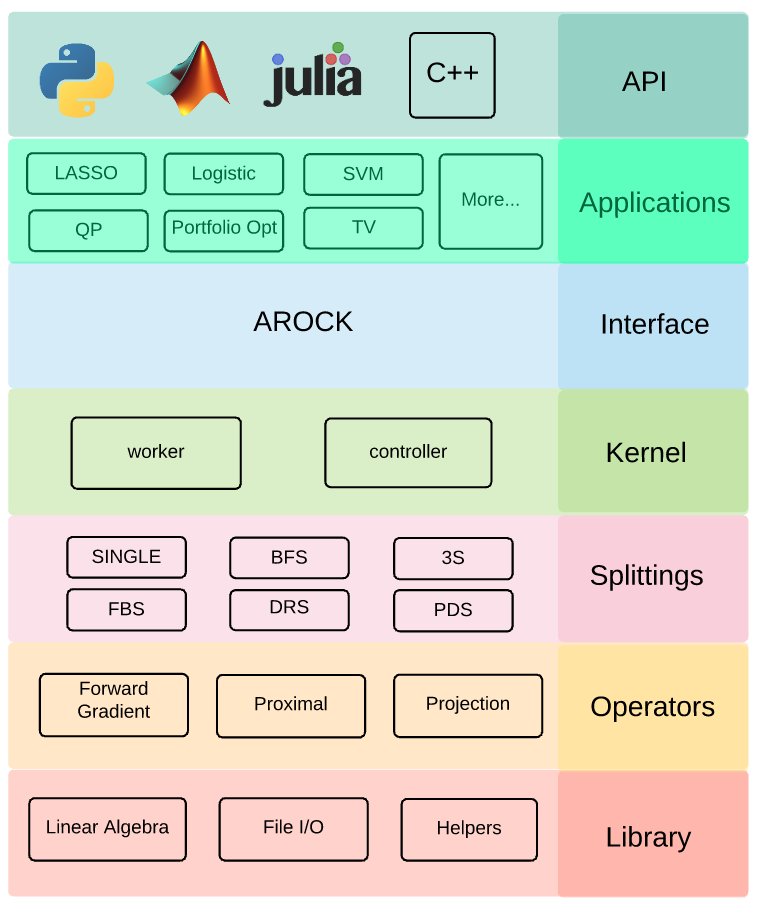
\includegraphics[width=0.45\textwidth]{./figs/architecture.png}
      \caption{Architectures for distributed memory systems. Linear algebra serves as the foundation for ARock. Other layers are structured according to the discussions in Section ??.}
        \label{fig:arch}
\end{figure}


\subsection{Library}
The library layer includes three major components: data structures and linear algebra functions, file I/O functions, and helper functions. The primary data structures are dense vector, dense matrix and sparse matrix. We implemented a few handy BLAS (Basic Linear Algebra Subprograms) wrappers. File I/O functions for matrices in the matrix market format\footnote{\url{http://math.nist.gov/MatrixMarket/formats.html}} and LIBSVM format\footnote{\url{https://www.csie.ntu.edu.tw/~cjlin/libsvmtools/datasets/}} are also implemented. Helper functions include a list of objective functions, command-line argument parsers, and error handling functions. Those functions are extensively used in the operator layer and the splitting layer. 

\subsection{Operators}
The operator layer is a library of projection operators, proximal operators and forward operators which are useful for high-level iterative algorithms. Currently, we implemented 17 operators. These operators are modularized and implemented in the form of \emph{function object (functor)}. 

In general, each operator struct has three overloaded parenthesis operators: one consumes a scalar and calculates the update; one takes a vector and an index then applies the coordinate update; one takes an input vector and an output vector, then performs full update to the input vector and saves the results in the output vector. Constructors and update cached variable function are also provided. If an operator involves data, pointers to the data are added as member variables. The following code is a template for implementing operators.
\begin{lstlisting}[language=C++]
struct operator_name {
  double step_size;  // operator related step size
  double weight;  // weight on the operator  
  double operator() (double val);  // scalar update operator  
  // coordinate update operator
  double operator() (Vector* v, int index = 0);  
  // full update operator
  void operator() (Vector* v_in, Vector* v_out); 
  // update cached variables
  void update_cache_vars(double old_x_i, double new_x_i, int i);
  operator_name();  // default constructor
  operator_name(argument list);  // customized constructor
};
\end{lstlisting}


\cut{
\begin{lstlisting}[language=c++]
  struct functor_name {
    // the step_size that associated with the operator  
    double step_size;
    // weight on the original function, e.g., f(x) = weight ||x||_1
    double weight;      
    // returns the operator evaluated on v at the given index
    double operator() (Vector* v, int index);
    // returns the operator evaluated on v at the given index
    double operator() (double val, int index);
    // full update
    void operator() (Vector* v_in, Vector* v_out);
    // (Optional) update the cached variables, it 
    // takes the old x_i and new x_i, updated at index.
    void update_cache_vars (double old_x_i, double new_x_i, int index);
    // update the step size. The step size might be
    // changed during the iterative process
    void update_step_size (double step_size_) {
      step_size = step_size_;
    }
    // customized constructor
    functor_name (double step_size_, double weight_ = 1.) :
        step_size(step_size_), weight(weight_) {}
    // default constructor
    functor_name () : step_size(0.), weight(1.) {}
  };
\end{lstlisting}
}

\subsection{Splitting Schemes}
Splitting schemes are templated on operators. Based on the discussions in Section \ref{sec:splitting}, we implemented several splitting schemes, including PPA, FBS, BFS and PRS. The structure of the splitting scheme has the following form. 
 \begin{lstlisting}[language=c++]
 template <typename Op1, typename Op2, ...>
 struct OperatorSplitting {
   double relaxation_step_size; 
   Vector* x;
   Op1 p1;  // define the operators
   // calculates the update of x at index
   double operator(int index);
   // update the operator related parameters
   void update_params(Params* params);
   // customized constructor
   OperatorSplitting(argument list);
};
\end{lstlisting}
It usually has one or more than one operators as the template arguments. It has an overloaded parenthesis operator which performs updates to the unknown variable $x$ and maintained variables. The update is carried out by calling appropriate member functions of the templated operators. An example of the implementation of the parenthesis operator for FBS is shown below. 
\begin{lstlisting}[language=c++]
  double operator() (int index) {
    // Step 1: read the old x[index]
    double old_x_at_idx = (*x)[index]; 
    // Step 2: local calculation
    double forward_grad_at_idx = forward(x, index);
    double val = backward(forward_grad_at_idx);
    double S_i = old_x_at_idx - val;
    // Step 3: get the most recent x[index] before updating it
    old_x_at_idx = (*x)[index];
    // Step 4: update x at index 
    (*x)[index] -= relaxation_step_size * S_i;    
    // Step 5: update the maintained variable Atx
    forward.update_cache_vars(old_x_at_idx, (*x)[index], index);
    return S_i;
  }
\end{lstlisting}



\subsection{Worker and Controller}
ARock consists of several workers and a controller. Each worker has access to the shared data, the maintained variables, the unknown parameter $x$, and other algorithm related constants. Each worker continuously updates some coordinates of $x$ until the stopping criterions are satisfied. The coordinates can be updated in a cyclic or random fashion. At the same time, workers share delay monitoring information and convergence progress information with the controller, who use the information to dynamically update the step sizes to facilitate the convergence of ARock. Figure~\ref{fig:worker_controller} demonstrates the relations of workers, controller, and shared memory.  
\begin{figure}[!h]
      \centering
        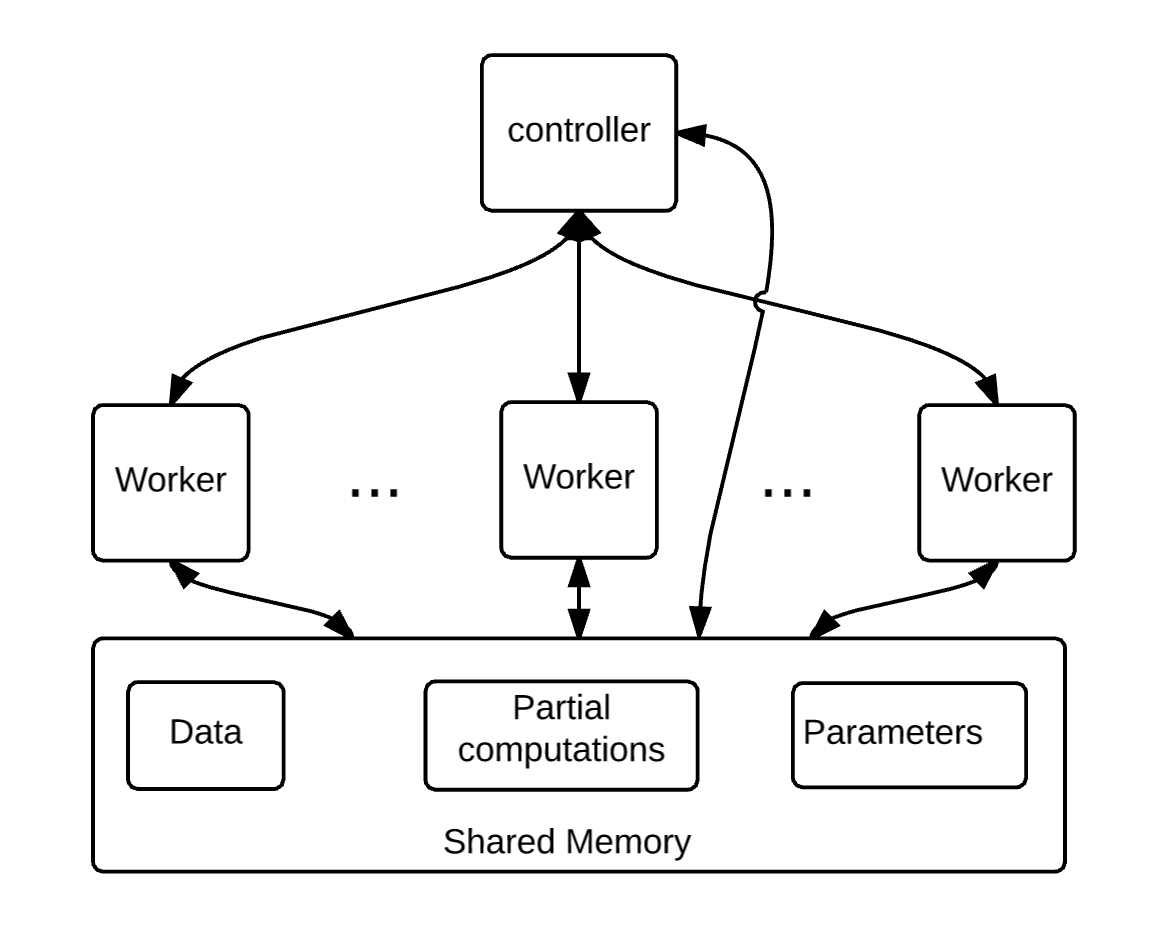
\includegraphics[width=0.5\textwidth]{./figs/worker_controller.png}
      \caption{Relationship between workers, controller and shared memory.}
        \label{fig:worker_controller}
\end{figure}

\subsection{ARock Interface}
The ARock interface simply spawns a set of threads with one thread taking the controller role and the rest of threads being the workers. The interface of ARock is the following. It takes three inputs, including a splitting scheme, a parameter structure and a controller.
\begin{lstlisting}[language=c++]
template<typename Splitting>
void AROCK(Splitting op, Params parameters, Controller<Splitting> controller);
\end{lstlisting}


\subsection{Applications}
Section \ref{sec:quick_start} gives an example of using ARock to solve the sparse logistic regression problem. Other applications are implemented or can be implemented similarly. We have implemented several applications from statistical machine learning and scientific computing with the ARock framework. The applications can be compiled into executable files, which can then be executed through the command-line interface. For an unimplemented application, if the necessary operators and splitting schemes are defined in the ARock library, then creating an async-parallel algorithm can be as simple as calling ARock on the appropriate splitting scheme. 




%% !TEX root = ./arock_pkg_main.tex
\section{The Fixed-point Problem}
\begin{enumerate}
\item the fixed-point problem;
\item cached variables;
\item and refer everything else to CF-paper;
\end{enumerate}


%% !TEX root = ./arock_pkg_main.tex
\section{Related Works}
\begin{enumerate}
\item review existing for serial implementation and theory of CU method (steel some from the CF paper);
\item review existing sync-parallel solvers, so far we are aware of the followings 
\begin{itemize}
\item ac-dc package: \url{https://github.com/optml/ac-dc}, 
\end{itemize}
\item review existing async-parallel solver:
\begin{itemize}
\item Passcode: \url{http://www.cs.utexas.edu/~rofuyu/exp-codes/passcode-icml15-exp/}
\item Hogwild: \url{http://i.stanford.edu/hazy/victor/Hogwild/}
\end{itemize}

\end{enumerate}


%% !TEX root = ./arock_pkg_main.tex
\section{Organization}
\begin{enumerate}
\item Introduction
\item The fixed-point problem
\item The software package
	\begin{enumerate}
	\item Practical usage;
	\item Documentation;
	\item Design;
	\end{enumerate}
\item Comparison;

\item Conclusion 

\item Appendix (derivation of the examples??)

\end{enumerate}



% % !TEX root = ./arock_pkg_main.tex
\section{User Interaction}

\begin{itemize}
\item Implement apps (using library);
\item Using synchronous;
\item Implement your own operator;
\item implement your own coordinate update (put the entire update to a single operator)
\end{itemize}


% !TEX root = ./arock_pkg_main.tex
\section{Numerical Experiments}
In this section, we illustrate the efficiency of ARock for three applications: elastic net regularized logistic regression, portfolio optimization,  and nonnegative matrix factorization.


% !TEX root = ./arock_pkg_main.tex
\subsection{Minimizing Elastic Net Logistic Regression}
In this subsection, we apply ARock with FBS to the elastic net regularized logistic regression problem
\begin{equation}\label{eqn:l12_log}
\Min_{x \in \mathbb{R}^n} \lambda_1 \|x\|_1 + \frac{\lambda_2}{2} \|x\|^2_2 + \sum_{i=1}^N \log\big(1 + \exp(-b_i \cdot a_i^T x)\big),
\end{equation}
where $\{(a_i, b_i)\}_{i=1}^N$ is the set of sample-label pairs, $\lambda_1=0.001$, $\lambda_2 = 1.$, and $n$ and $N$ represent the numbers of features and samples, respectively. This test uses two libsvm datasets\footnote{\url{http://www.csie.ntu.edu.tw/~cjlin/libsvmtools/datasets/}}: news20, and url.

Figure \ref{fig:log_reg_obj} gives the running times of  the full update (sync-parallel) and ARock (async-parallel) implementations on the two datasets. Figure~\ref{fig:log_reg_speedup} is the speedup performance comparison of the two methods. We can observe that ARock achieves approximate-linear speedup, but sync-parallel scales poorly as we explain below. One can also see that ARock converges faster due to more relaxed forward operator step size selection. 

In the sync-parallel implementation,  all the running cores have to wait for the last core to finish an iteration, and therefore if a core has a large load, it slows down the iteration. Although every core is (randomly) assigned to roughly the same number of features at each iteration, their  $a_i$'s have very different numbers of nonzeros, and the core with the largest number of nonzeros is the slowest (Sparse matrix computation is used for both datasets, which are very large.) As more cores are used,  despite that they altogether do more work at each iteration,  the per-iteration time reduces as the slowest core tends to be slower.


\begin{figure}[!h]
        \centering
       \begin{subfigure}[b]{0.4\textwidth}
                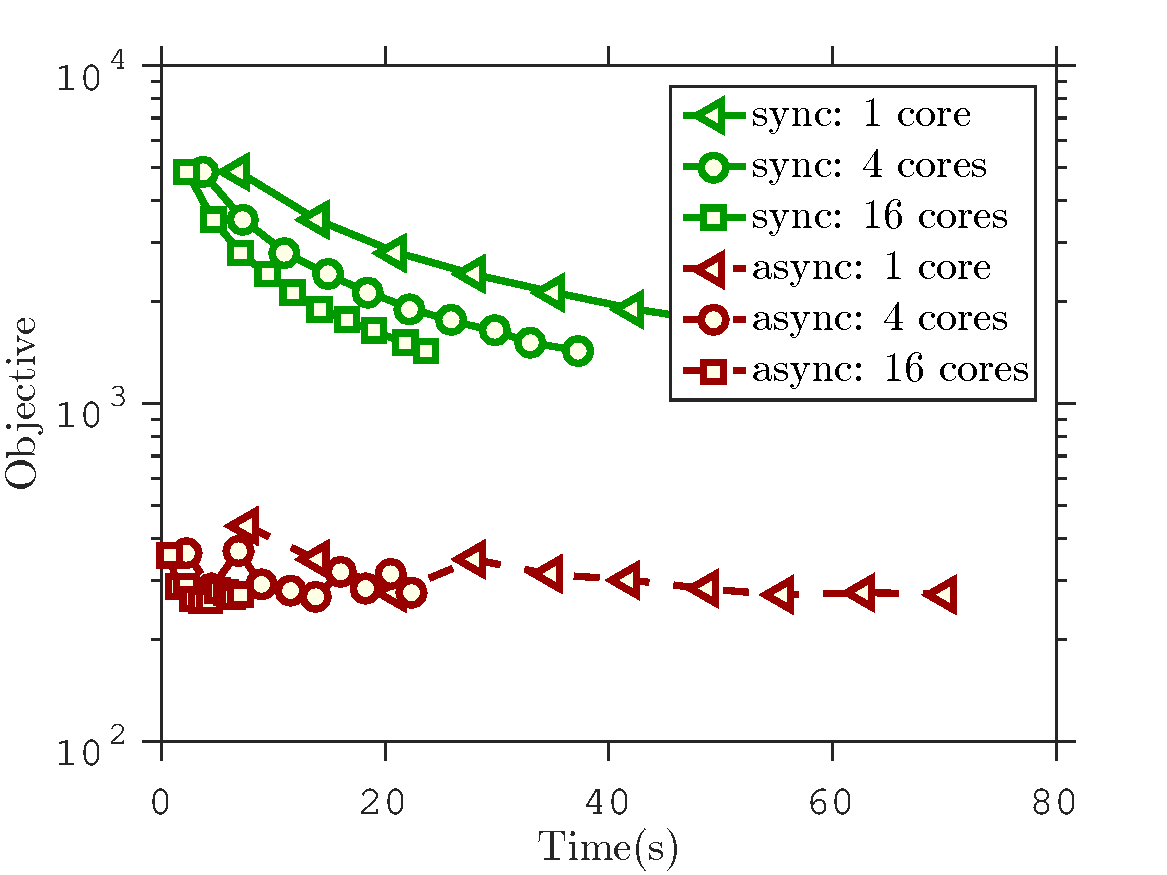
\includegraphics[width=\textwidth]{./figs/news20_obj}
                \caption{news20}
        \end{subfigure}
        ~~
        \begin{subfigure}[b]{0.4\textwidth}
                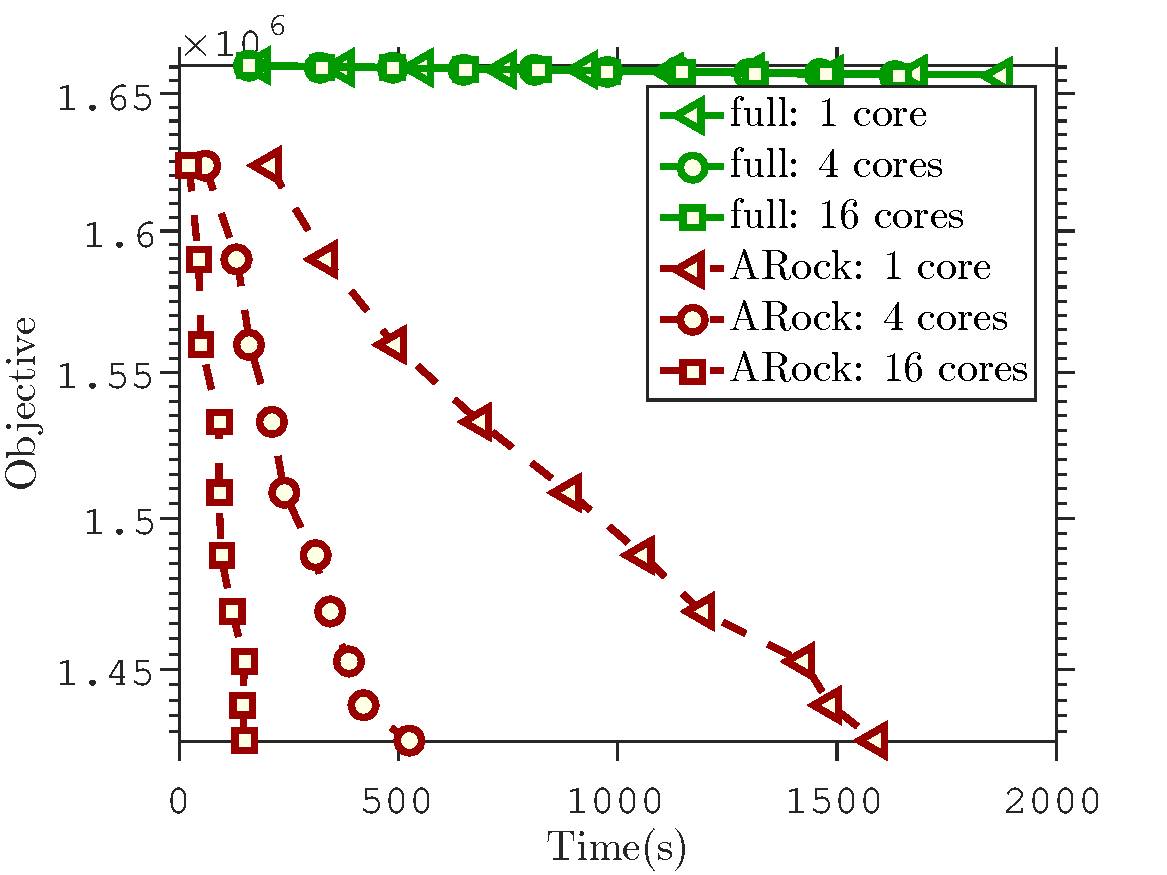
\includegraphics[width=\textwidth]{./figs/url_obj}
                \caption{url}
        \end{subfigure} 
        \caption{Objective vs wall clock time.}\label{fig:log_reg_obj}
\end{figure}

\begin{figure}[!h]
        \centering
       \begin{subfigure}[b]{0.35\textwidth}
                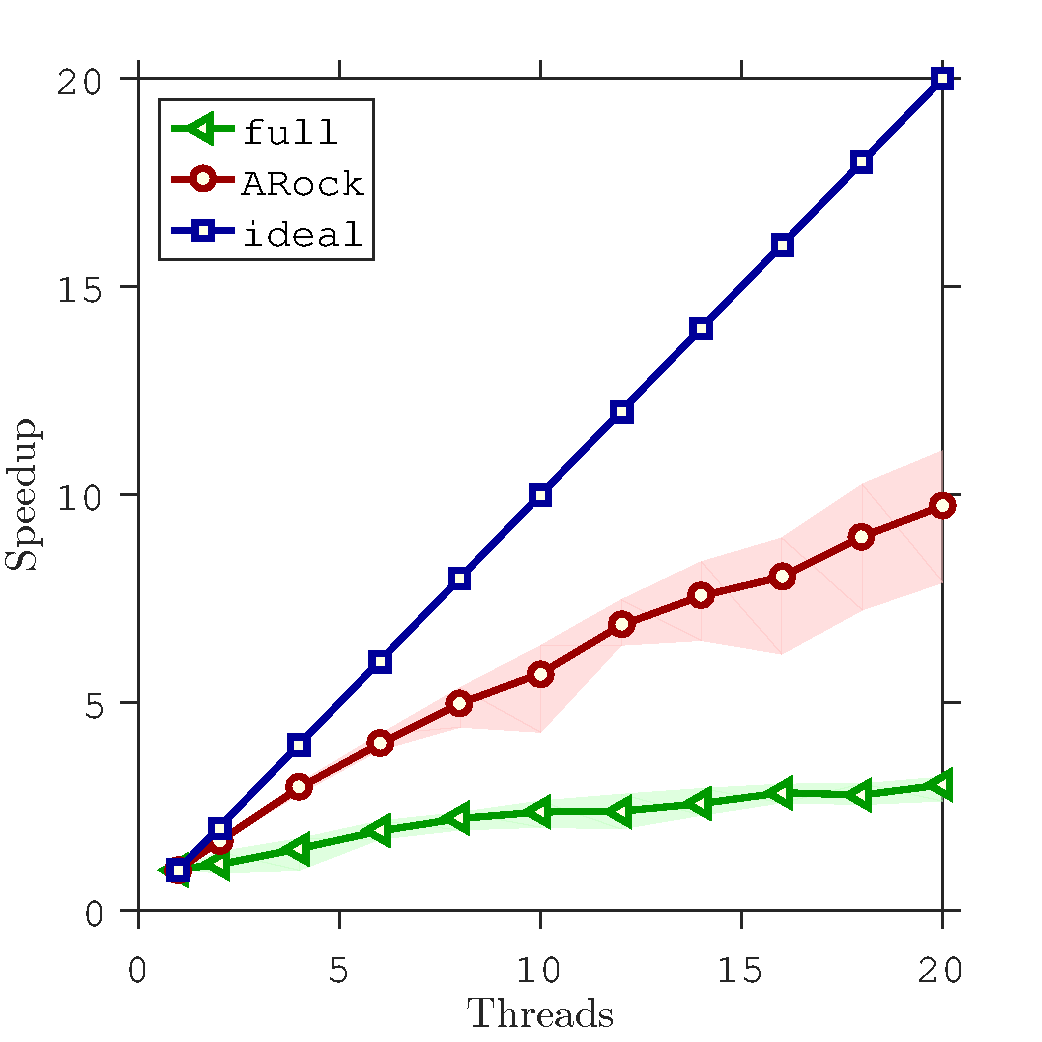
\includegraphics[width=\textwidth]{./figs/news20_speedup}
                \caption{news20}
        \end{subfigure}
        ~~
        \begin{subfigure}[b]{0.35\textwidth}
                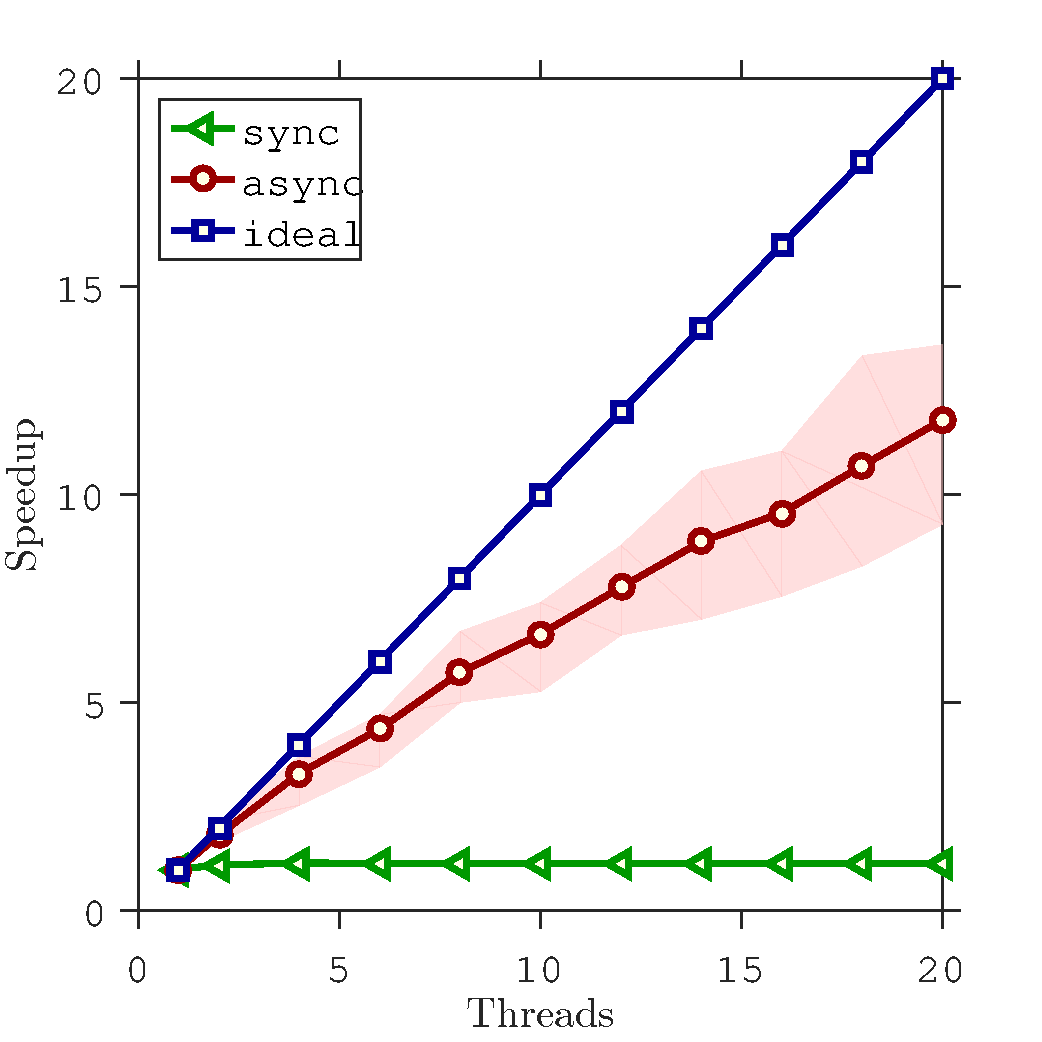
\includegraphics[width=\textwidth]{./figs/url_speedup}
                \caption{url}
        \end{subfigure}        
        \caption{Speedup vs number of threads.}\label{fig:log_reg_speedup}
\end{figure}

% !TEX root = ./arock_pkg_main.tex
\subsection{Portfolio Optimization}
% !TEX root = ./arock_pkg_main.tex
\subsection{Nonnegative matrix factorization}

We consider the following Nonnegative Matrix Factorization problem

\begin{equation*}
	\Min_{X \geq 0,Y \geq 0} ~\|A-X^T Y\|_2^2,
\end{equation*}
where $A \in \RR^{m\times n}$, $X \in \RR^{k \times m}$ and $Y \in \RR^{k \times m}$.
This problem, despite being nonconvex, has a special form.
The objective function is block multiconvex\footnote{the objective function is convex with respect to each variable when others are fixed} and its regularizers are separable. Problems of this type have been shown \citep{XuYin2013_block,XuYin2014_GloballyConvergent,BolteSabachTeboulle2014_proximal} to be amenable to coordinate update techniques and further amenable \citep{2016APALM} to the asynchronous regime.
As the problem is nonconvex, convergence is given to a local minimizer, not a global minimizer.

We run TMAC on a synthetic problem, $A=\hat X^T \hat Y$ ,  with $m=1000$ and $k=20$.
Elements of $\hat X$ and $\hat Y$ sampled independently from $N(0, 1)$ normal distribution, then threshold positive.
We ran the tests with variable number of threads and iterations.
The following results are the averages resulting from 20 runs.


\begin{figure}[!h]
        \centering
       \begin{subfigure}[b]{0.4\textwidth}
                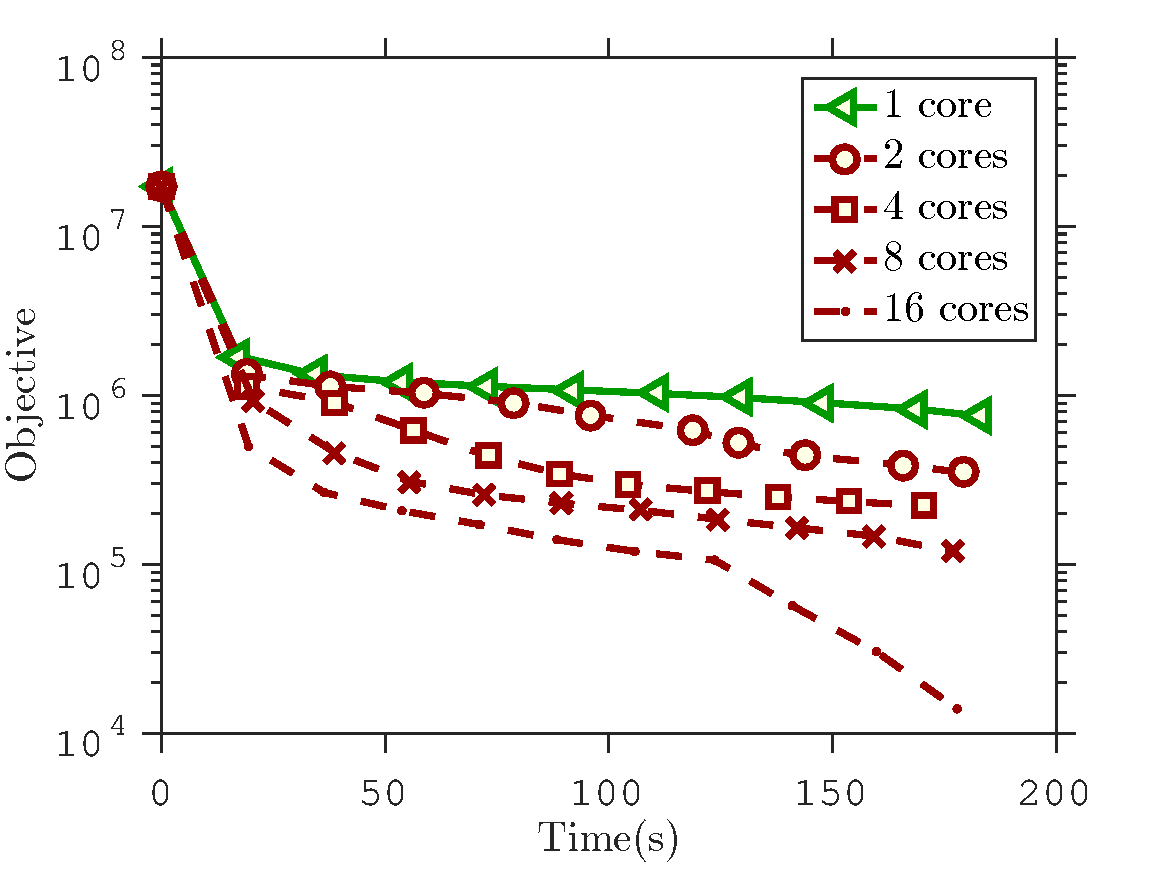
\includegraphics[width=\textwidth]{./figs/NMF_plot}
                \caption{Objective vs walll clock time}
        \end{subfigure}
        ~~
        \begin{subfigure}[b]{0.4\textwidth}
                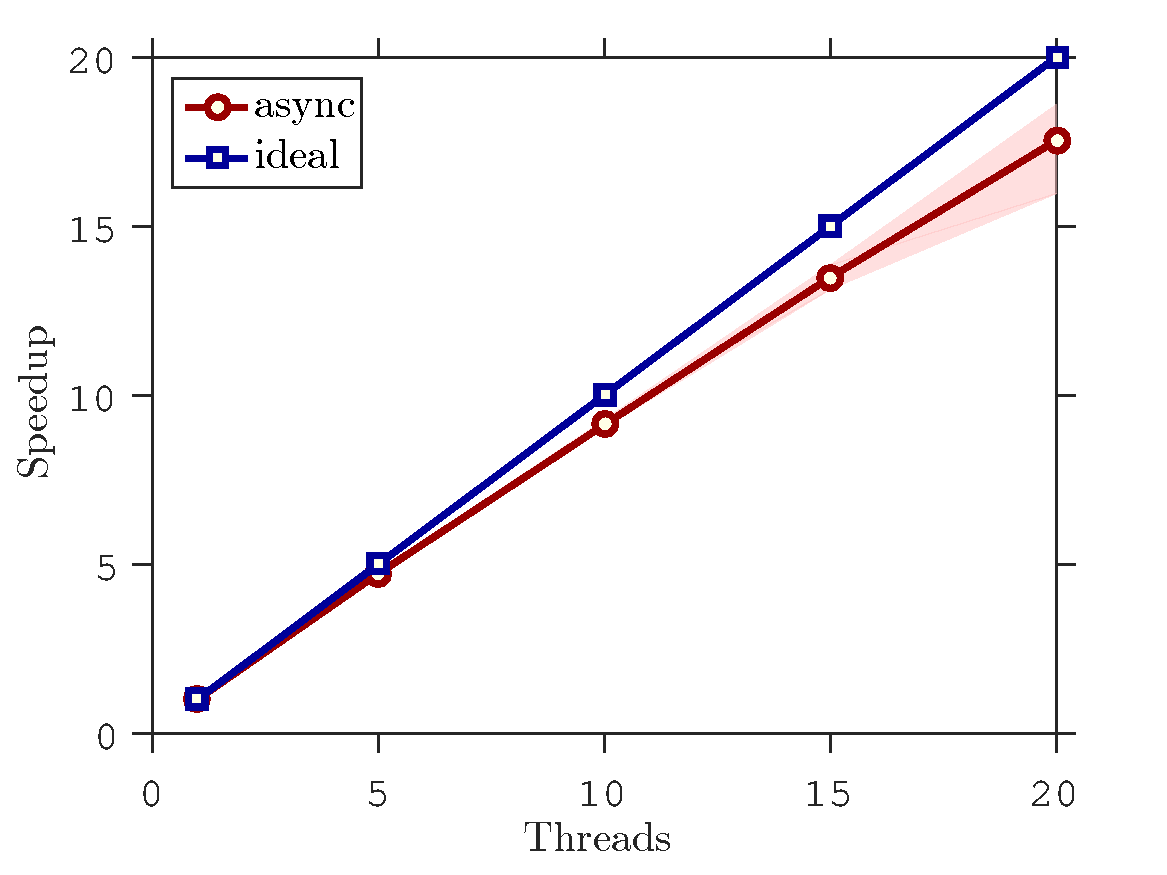
\includegraphics[width=\textwidth]{./figs/speedup}
                \caption{speedup}
        \end{subfigure}
        \caption{NMF results}\label{fig:NMF_speedup}
\end{figure}


To show scalability we increased the dimension of $k$, and tested the speedup.
\begin{table}[!h]
\centering
\begin{tabular}{rrrr}
 \toprule
{threads}&{k=10}&{k=20}&{k=100}\\\cmidrule{1-4}
1&1.00&1.00&1.00\\%\hline
2&1.97&1.98&1.98\\%\hline
4&3.75&3.75&3.76\\%\hline
8&7.12&7.33&7.35\\%\hline
16&13.38&14.51&14.43\\%\hline
\bottomrule
\end{tabular}
 \caption{\label{tab:nmf_res}Speedup results for nonnegative matrix factorization. }
\end{table} 
% !TEX root = ./arock_pkg_main.tex
\subsection{Minimizing Huber Loss}

% !TEX root = ./arock_pkg_main.tex
\subsection{Minimizing Elastic Net Logistic Regression}
In this subsection, we apply ARock with FBS to the elastic net regularized logistic regression problem
\begin{equation}\label{eqn:l12_log}
\Min_{x \in \mathbb{R}^n} \lambda_1 \|x\|_1 + \frac{\lambda_2}{2} \|x\|^2_2 + \sum_{i=1}^N \log\big(1 + \exp(-b_i \cdot a_i^T x)\big),
\end{equation}
where $\{(a_i, b_i)\}_{i=1}^N$ is the set of sample-label pairs, $\lambda_1=0.001$, $\lambda_2 = 1.$, and $n$ and $N$ represent the numbers of features and samples, respectively. This test uses two libsvm datasets\footnote{\url{http://www.csie.ntu.edu.tw/~cjlin/libsvmtools/datasets/}}: news20, and url.

Figure \ref{fig:log_reg_obj} gives the running times of  the full update (sync-parallel) and ARock (async-parallel) implementations on the two datasets. Figure~\ref{fig:log_reg_speedup} is the speedup performance comparison of the two methods. We can observe that ARock achieves approximate-linear speedup, but sync-parallel scales poorly as we explain below. One can also see that ARock converges faster due to more relaxed forward operator step size selection. 

In the sync-parallel implementation,  all the running cores have to wait for the last core to finish an iteration, and therefore if a core has a large load, it slows down the iteration. Although every core is (randomly) assigned to roughly the same number of features at each iteration, their  $a_i$'s have very different numbers of nonzeros, and the core with the largest number of nonzeros is the slowest (Sparse matrix computation is used for both datasets, which are very large.) As more cores are used,  despite that they altogether do more work at each iteration,  the per-iteration time reduces as the slowest core tends to be slower.


\begin{figure}[!h]
        \centering
       \begin{subfigure}[b]{0.4\textwidth}
                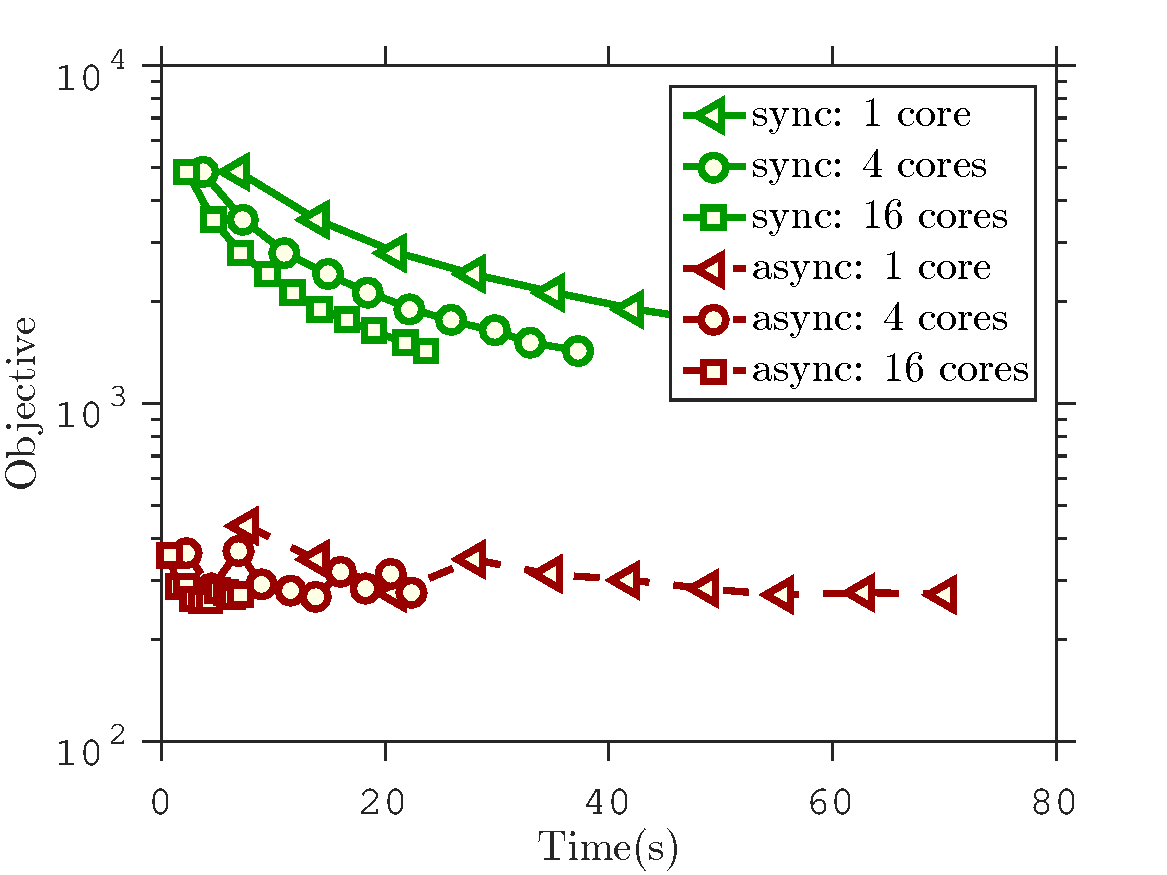
\includegraphics[width=\textwidth]{./figs/news20_obj}
                \caption{news20}
        \end{subfigure}
        ~~
        \begin{subfigure}[b]{0.4\textwidth}
                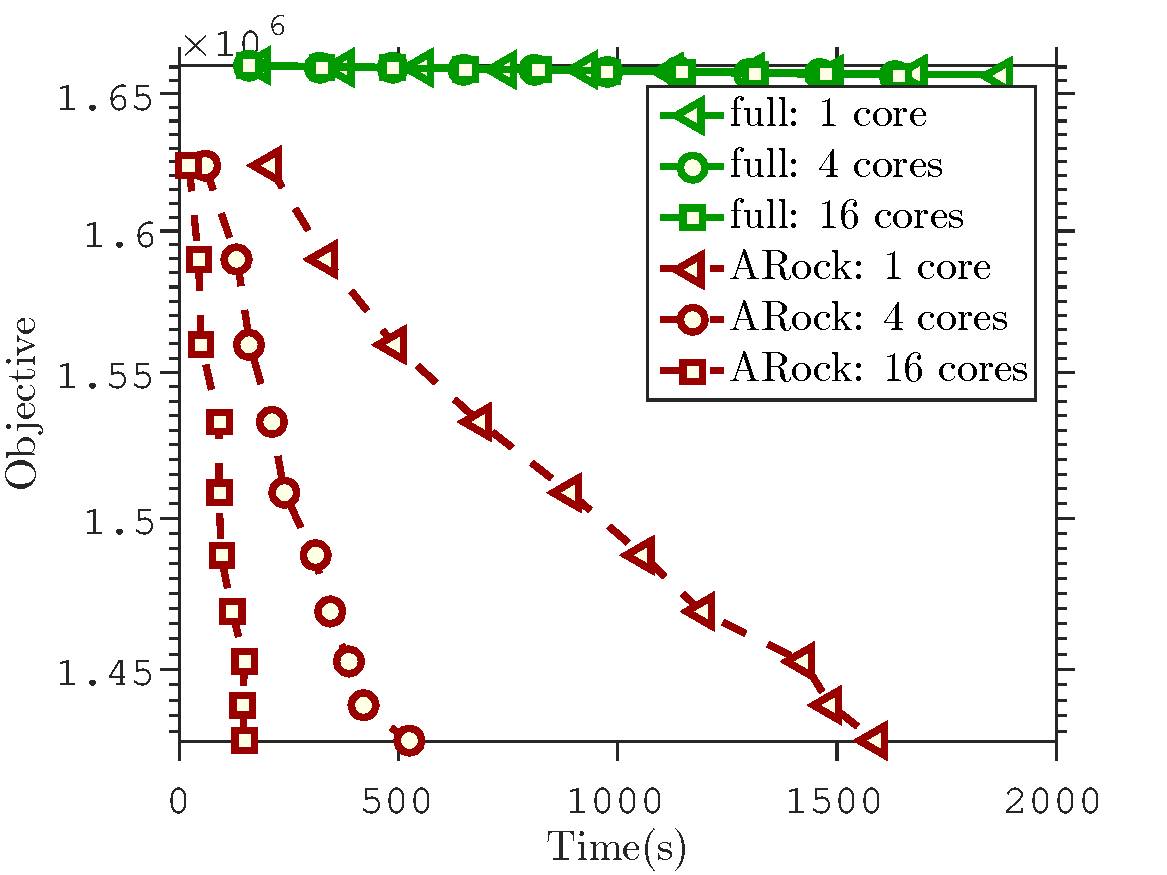
\includegraphics[width=\textwidth]{./figs/url_obj}
                \caption{url}
        \end{subfigure} 
        \caption{Objective vs wall clock time.}\label{fig:log_reg_obj}
\end{figure}

\begin{figure}[!h]
        \centering
       \begin{subfigure}[b]{0.35\textwidth}
                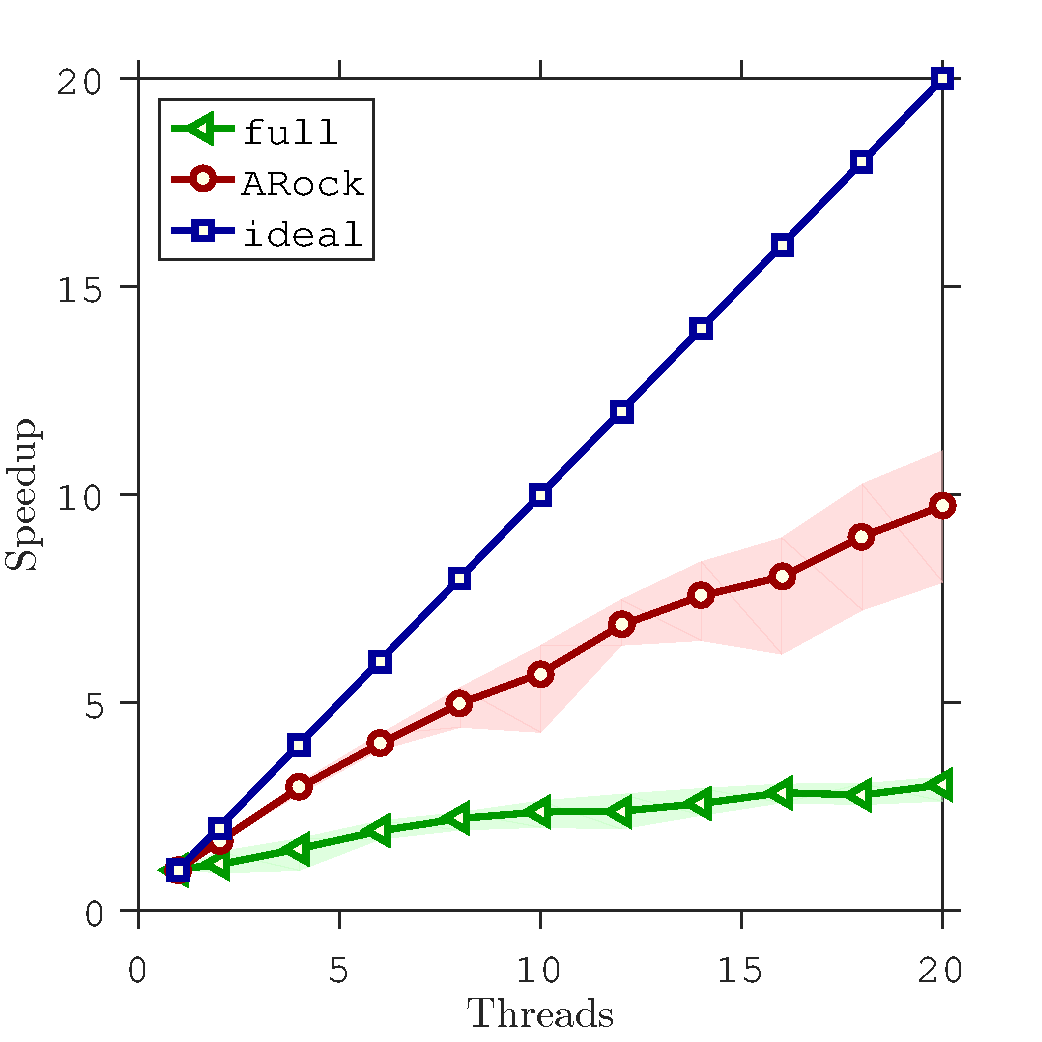
\includegraphics[width=\textwidth]{./figs/news20_speedup}
                \caption{news20}
        \end{subfigure}
        ~~
        \begin{subfigure}[b]{0.35\textwidth}
                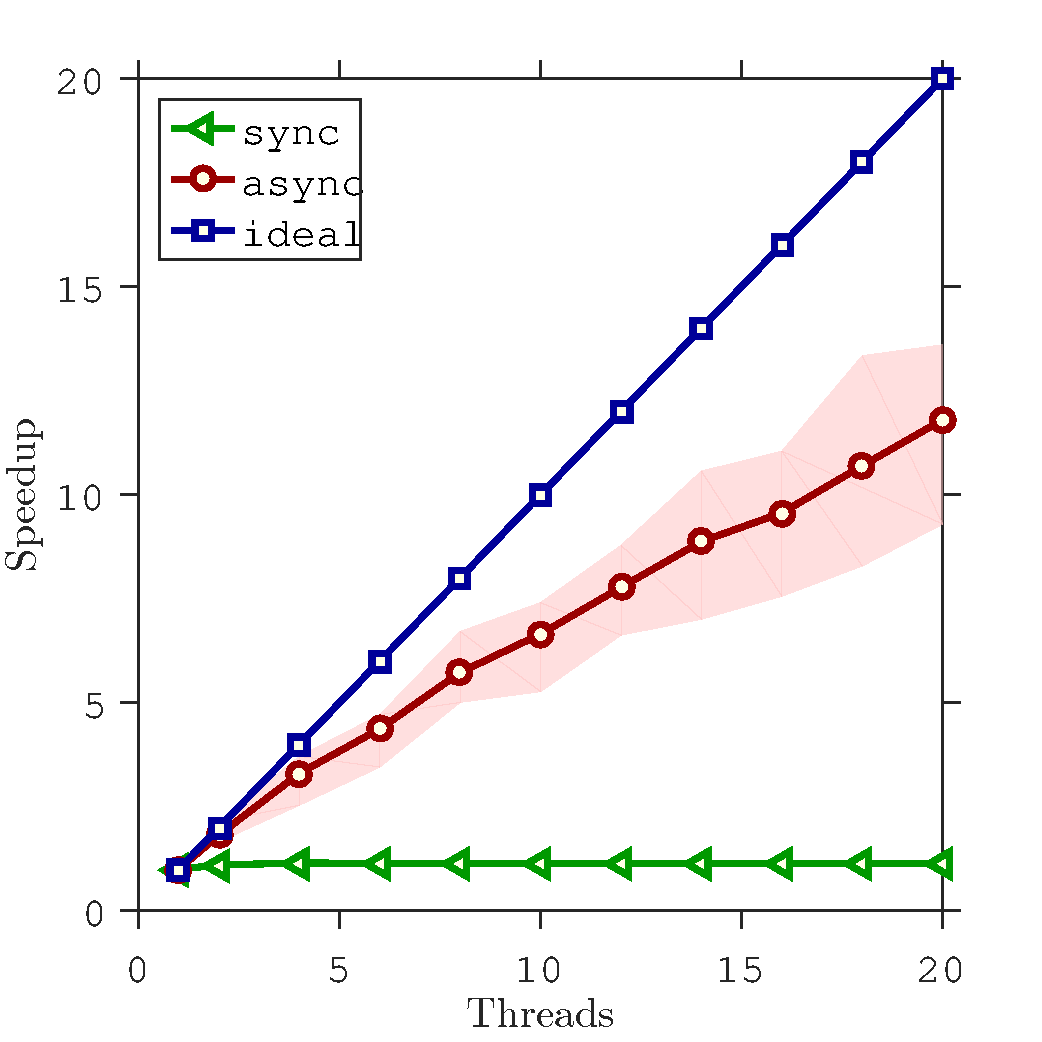
\includegraphics[width=\textwidth]{./figs/url_speedup}
                \caption{url}
        \end{subfigure}        
        \caption{Speedup vs number of threads.}\label{fig:log_reg_speedup}
\end{figure}

% !TEX root = ./arock_pkg_main.tex
\subsection{Portfolio Optimization}
% !TEX root = ./arock_pkg_main.tex
\subsection{Nonnegative matrix factorization}

We consider the following Nonnegative Matrix Factorization problem

\begin{equation*}
	\Min_{X \geq 0,Y \geq 0} ~\|A-X^T Y\|_2^2,
\end{equation*}
where $A \in \RR^{m\times n}$, $X \in \RR^{k \times m}$ and $Y \in \RR^{k \times m}$.
This problem, despite being nonconvex, has a special form.
The objective function is block multiconvex\footnote{the objective function is convex with respect to each variable when others are fixed} and its regularizers are separable. Problems of this type have been shown \citep{XuYin2013_block,XuYin2014_GloballyConvergent,BolteSabachTeboulle2014_proximal} to be amenable to coordinate update techniques and further amenable \citep{2016APALM} to the asynchronous regime.
As the problem is nonconvex, convergence is given to a local minimizer, not a global minimizer.

We run TMAC on a synthetic problem, $A=\hat X^T \hat Y$ ,  with $m=1000$ and $k=20$.
Elements of $\hat X$ and $\hat Y$ sampled independently from $N(0, 1)$ normal distribution, then threshold positive.
We ran the tests with variable number of threads and iterations.
The following results are the averages resulting from 20 runs.


\begin{figure}[!h]
        \centering
       \begin{subfigure}[b]{0.4\textwidth}
                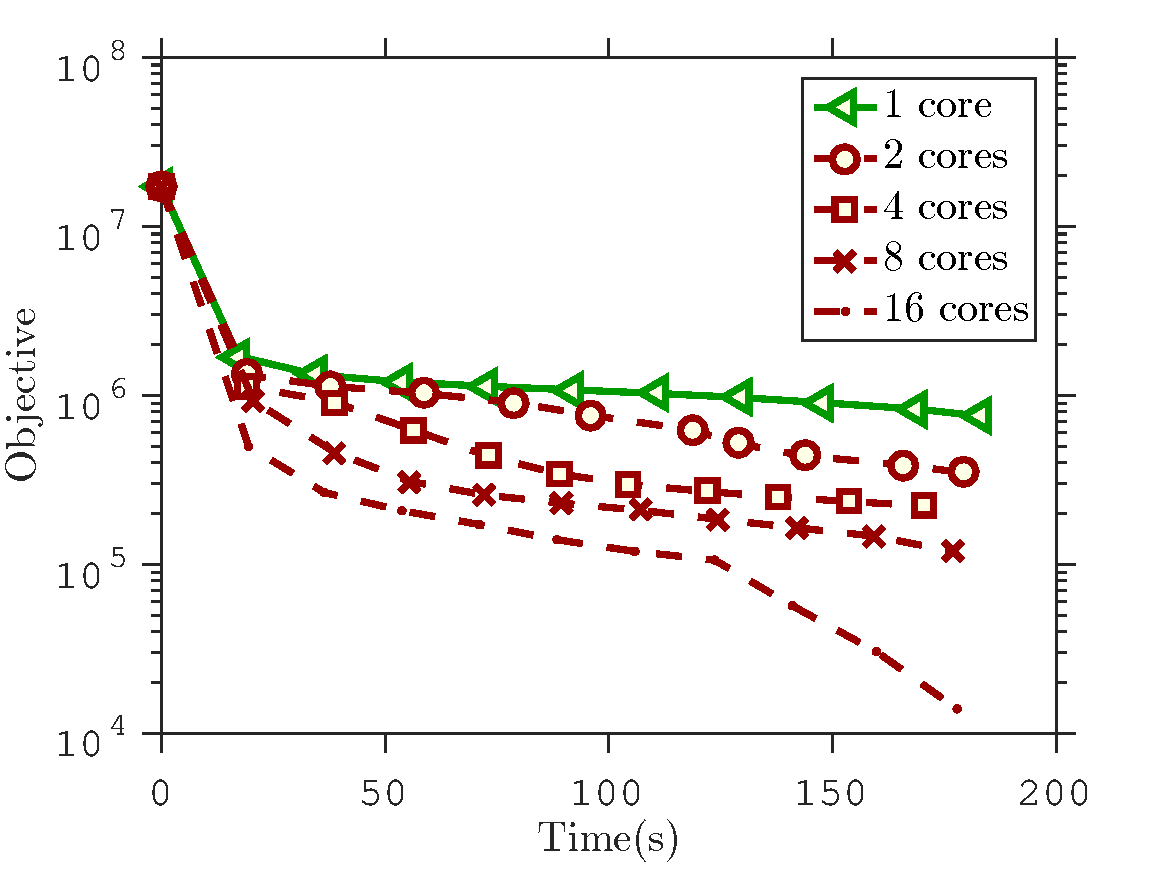
\includegraphics[width=\textwidth]{./figs/NMF_plot}
                \caption{Objective vs walll clock time}
        \end{subfigure}
        ~~
        \begin{subfigure}[b]{0.4\textwidth}
                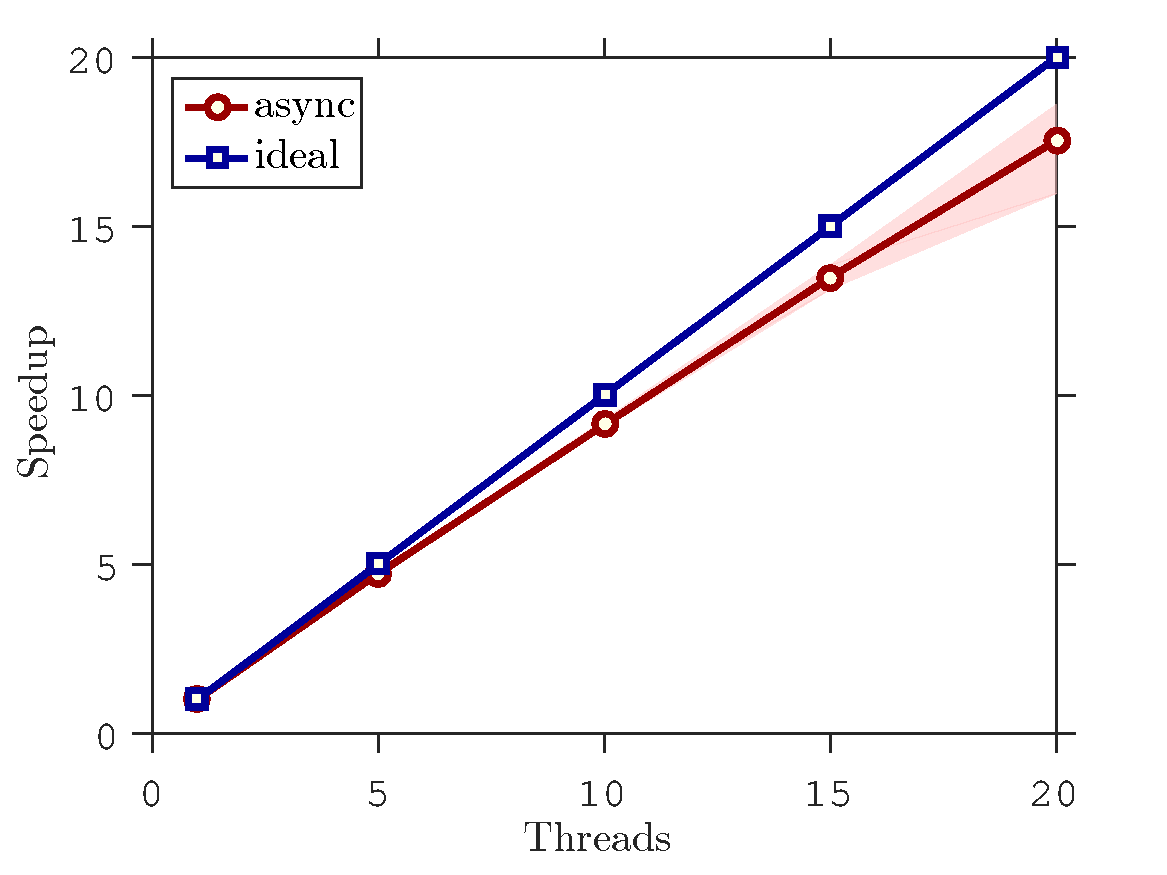
\includegraphics[width=\textwidth]{./figs/speedup}
                \caption{speedup}
        \end{subfigure}
        \caption{NMF results}\label{fig:NMF_speedup}
\end{figure}


To show scalability we increased the dimension of $k$, and tested the speedup.
\begin{table}[!h]
\centering
\begin{tabular}{rrrr}
 \toprule
{threads}&{k=10}&{k=20}&{k=100}\\\cmidrule{1-4}
1&1.00&1.00&1.00\\%\hline
2&1.97&1.98&1.98\\%\hline
4&3.75&3.75&3.76\\%\hline
8&7.12&7.33&7.35\\%\hline
16&13.38&14.51&14.43\\%\hline
\bottomrule
\end{tabular}
 \caption{\label{tab:nmf_res}Speedup results for nonnegative matrix factorization. }
\end{table} 

% !TEX root = ./arock_pkg_main.tex
\section{The Software Package}

% !TEX root = ./arock_pkg_main.tex
\subsection{Practical Usage}
\begin{itemize}
\item download;
\item script for downloading the required packages; 
\item script to do prepackage solvers;
\end{itemize}



% !TEX root = ./arock_pkg_main.tex
\subsection{Documentation}
\begin{itemize}
\item html docs;
\item heavily commented code; 
\item example code;
\item youtube HOWTO;
\end{itemize}


% !TEX root = ./arock_pkg_main.tex
\section{Architecture}

Writing efficient code is is very different from writing an optimization algorithm.
Our toolbox's architecture is designed to mimic how a scientist writes down an optimization algorithm.
The toolbox achieves this by separating into the following layers: Numerical Linear Algebra, Operator, Scheme, Kernel, and Multicore Driver.
Each layer represents a different mathematical component of a multicore optimization algorithm. 

The following is a brief description of each layer and how it interacts with the layers above and below it.

\subsection{Numerical Linear Algebra}

We use eigen, Sparse BLAS, and BLAS in our Toolbox.
Directly using efficient numerical packages like BLAS can be intimidating due to complex function calls. We provide simplified function calls for common linear algebra operations like $a_i^T x$ in Algorithm \ref{alg:fbs_l1_log}. This layer insulates the user from the grit of raw numerical implementation. Higher layers use the Numerical Linear Algebra Layer in their implementations.

If our provided functions are not sufficient, documentation for eigen, Sparse BLAS, and BLAS can be found in the following locations. As our codebase is growing, opening an issue on the github is suggested as well.

\subsection{Operator}

The Operator layer contains Forward Operator objects(gradient steps) and Backward Operator (proximal mappings) objects. These Operators types see heavy reuse throughtout optimization.
For instance, Algorithm \ref{alg:fbs_l1_log}, along with any other gradient based method for sparse logistic regression, requires the computation of the Forward Operator $x - \eta \, \nabla \,\sum_{i = 1}^m \log (1 + \exp(-b_i \cdot a_i^T x))$. On a similar vein, Nonnegative Matrix Factorization and Nonnegative Least Squares share a backwad operator, the projection onto the positive orthant.

Much as the Numerical Linear Algebra Layer insulates the user from the computation details of numerical linear algebra, the Operator layer insulates the user from the computational details of Operators. This is achieved by encapsulating the computation of common Forward and Backward Operators into Operator objects. The Operator layer, as a result, allows users to reason and code at the level of Operators. Higher Layers use Operator objects as components in the creation of algorithms.

In the case that an Operator outside of the provided Operators is needed, the user can implement their own. See section about implementation?
 
{\color{red} Implementation detail, possibly move to dedicated section?} As our Toolbox is designed for coordinate update methods, each Operator is implemented to compute coordinates efficiently. A coordinate or block of coordinates can be computed efficienty if the computational cost of a single coordinate or a block of coordinates of the operator is reduced by a dimensional factor compared to the evaluation of the entire operator (ex: $(Ax)_i$ versus $Ax$). In some cases cacheing, the storing an intermediate computation, can improve the efficiency of a coordinate block (ex: $(A^TAx)_i$ versus $(ATy)_i$ where $y=Ax$). These ideas are formalized in CFU paper.  In the case that a Operator is needed that we have not implemented, a user can use CFU paper as a guide to  implementing their own Operator.
 

\subsection{Scheme}

Objects in the Scheme Layer are designed to mimic the process of applying an optimization method to a problem.
For example, \eqref{eq:fbs_l1_log} is Forward Backward Splitting (also referred as Proximal Gradient Method) applied to a specific problem, sparse logistic regression.
Forward Backward Splitting was applied to sparse logistic regression by specifying Forward and Backward Operators.
So to is the case with Scheme objects.
Each object in the Scheme layer contains an optimization method.
It is specialized to a problem by specifying Operators. We can see this in code snippet above {\color{red} Need a way to reference the code snippet, can we embed in a figure?}.
The scheme object \texttt{fbs} is specialized to sparse logistic regression by specifying its type as \texttt{ForwardBackwardSplitting<forward\_grad\_for\_log\_loss<SpMat>, prox\_l1>}.
  
We provide implemenations of the following schemes: Forward Backward Splitting, Proximal Point Method,  Gradient Descent, Backward Forward Splitting, and Peaceman-Rachford Splitting.
If the provided schemes are not sufficient, the user may implement their own scheme.
The user is encouraged to use objects from the Operator Layer as building blocks, but direct implementaiton using the Linear Algebra Layer is perfectly functional.



{\color{red} implementation details, move to another section}

Objects in the Scheme Layer are implemented as templates.
Templates, in C++, are rules for generating an object.
Based upon the arguments passed to the template, C++ automatically constructs a corresponding object type for the user.
For example, in code snippet \ref{fbs_l1_log_code} the scheme type of \texttt{fbs} is defined by the arguments to the forward backward splitting template, \texttt{forward\_grad\_for\_log\_loss<SpMat>}, and \texttt{prox\_l1}. 
Different arguments to the template result in different coordinate update schemes.


\begin{lstlisting}[language=C++]
struct Scheme_Interface {
void update_params(Params* params);
double operator() (int index);
};
\end{lstlisting}

\subsection{Kernel}

Agents, in our Toolbox, are realized as threads. 
C++11 threads are created from functions.
The Kernel Layer contains the functions used to create agents. 
As can be seen in algorithm \ref{alg:fbs_l1_log}, 
an agent chooses an coordinate according to some rule and combines the coordinate with a scheme object to produce an update.
For each coordinate choice rule, there is a corresponding function.
We provide the following coordinate choice rules: cyclic, block cyclic, and randomized block. 
If the user desires a different coordinate rule, they may implement their own function. 

\subsection{Multicore Drivers}

The Multicore Driver layer is responsible for executing the Multicore algorithm. A Multicore Driver maps an object from the Scheme layer to agents.

of create threads (corresponding to agents in algorithm \ref{alg:fbs_l1_log}).
Consider algorithm \ref{alg:fbs_l1_log}.
The algorithm assumes the existence of computing agents.
The Multicore Driver layer is responsible for the creation and management of agents.
Decisions such as what coordinate rule, how many iterations, and stepsize are passed to the Multicore Driver through a Params object.

 If a controller (see later) is used, then a thread for the controller will also be created. When a thread is created, the layer grants it access to certain coordinates. Both thread creation and coordinate access are determined by the user-specified coordinate update scheme. For example, if the user specifies the random parallel scheme and ten threads, then ten threads (or nine threads plus a controller thread) will be created and each will  be granted to access all the coordinates (the ``random" selection rule will be passed to threads). Other schemes such as block-cyclic parallel, Gauss-Seidel parallel, as well as single-threaded schemes are implemented, too. 

This layer is also responsible for waiting for all threads to complete before returning the result to the user and terminating the algorithm.    

Therefore, this layer can be understood as a mapping from a coordinate update scheme to a thread manager. Note that this layer leaves the operations inside each thread to the other layers. As such, any user-specified operators, splitting scheme, and parameters are passed transparently to the next layer.

Most users can treat this layer as a black box. Only when a new coordinate update scheme or a new way to generate threads is desired, does the user need to make modifications to the code of this layer.



Interfaces are used when necessary. 
Interfaces are a set of assumed functionality of a layer.
Layers interact through their interfaces.
Consider the Interface for the Operator object:

\begin{lstlisting}[language=C++,label={Operator_Interface}]
struct Operator_Interface {
   // returns the operator evaluated on v at the given index
   double operator() (Vector* v, int index);
  // returns the operator evaluated on v at the given index
   double operator() (double val, int index);
  //applies full operator to v_in and write it to v_out
   void operator() (Vector* v_in, Vector* v_out);
  //optional: see CFU paper
  void update_cache_vars (double old_x_i, double new_x_i, int index);
  // update the step size
   void update_step_size (double step_size_) ;
 };
\end{lstlisting}

For an object to belong to the Operator layer, it must have these functions defined.
Attempting to use an object as an Operator that does not have the functionality defined by the Operator Interface will result in compiler errors.
Note that the Operator Inteface only includes the function declarations, not the implementation of the functions themselves.
As a result, implementation is decoupled from usage.
This allows for easy maintenance and specialization of code while not affecting the user's code.



% !TEX root = ./arock_pkg_main.tex
\section{Future Work}

New features are still being added to pkg. The following are some of the features we are exploring.

\subsection{Stochastic algorithms} 

Stochastic algorithms exploit summative structures in problems to produce cheap updates. Our current Toolbox does not currently support stochastic algorithms, but can be modified to do so. Such a modification would require stochastic operators. A developement branch will appear on our github.  

\subsection{Cluster computing}
 
 Currently, agents are realized as threads.
 This limits our toolbox to the multicore regime.
 Future releases intend to use MPI to bring \pkg~ to cluster computing. The new functionality will be provided in the Driver and the Kernel Layer. 

\subsection{User interface}
 \pkg~ requires the user to either use our prepackaged executables, or code moderately in C++.
 A graphic user interace is in development for those who wish avoid interacting directly with C++.
 This will limit the user to built-in functionality.
 In addition, interfaces to Matlab and Python will be provided for algorithms of particular interest.
 
\subsection{Automatic parameter choice}
\pkg~ requires the user to choose stepsizes, and number of threads.
In future releases we intend to provide automatic stepsize heuristics. 
Optimizing thread number is a function of current processor usage and computing architecture. 
We intend to provide functions to survey the current architecture and suggest proper levels of parallelism and asynchrony.

\subsection{Block coordinate update}
  Currently \pkg~ does not currently support block coordinate updates (updates consisting of a set of coordinates). Block coordinate updates present a tradeoff between iteration complexity and communication efficiency.
  Automatic block size deduction and block composition (the coordinates forming a block) is an open question.
We plan to explore several heuristics.

\subsection{New fields}

Splitting methods have been used in many fields (see "Some Facts about Operator-Splitting and
Alternating Direction Methods" for a more in depth discussion).
Our current release focuses on optimization, but provides a strong foundation for branching into other fields.
Fruitful fields to explore include:

\begin{itemize}
\item Time varying systems such as initial value problems and partial differential equations
\item Numerical simulations
\item Large scale numerical linear algebra 
\end{itemize}


\section{Conclusion }
We have developed \pkg, an easy-to-use open source toolbox for large scale optimization problems.
The toolbox implemented both sequential and parallel algorithms based on operator splitting methods, stochastic methods,
and coordinate update methods. The architecture of \pkg~is separated into several layers and mimics how a scientist writes down an optimization algorithm. Therefore, it is easy for one to obtain a new algorithm by modifying just one of the layers such as adding a new operator.


New features and applications will be added to \pkg~based upon new research and community input. The software and user guide \repo~ will be kept up-to-date and supported.


\bibliographystyle{siam}
\bibliography{asyn}

\end{document}
